\documentclass[twoside]{report}

\usepackage{tfg}

\makeglossaries

\begin{document}
	
	% PORTADA E INFORMACIÓN INICIAL
	\thispagestyle{empty}
\BgThispage

\begin{tikzpicture}[remember picture, overlay]
  \node[yshift=-5cm] at (current page.north west)
  {
    \begin{tikzpicture}[remember picture, overlay]
      \draw[fill = headingPortadaTFG, headingPortadaTFG, fill opacity = 1] (0,0) rectangle (\paperwidth,5cm);
      \node[yshift = 3cm, xshift = 0.5\paperwidth, font = \Huge, text centered, midway] {\color{textoHeadingPortadaTFM}\textbf{\universidad}};
      \node[yshift = 2cm, xshift= 0.5\paperwidth, font = \Huge, text centered, midway] {\color{textoHeadingPortadaTFM}\textbf{\escuela}};
    \end{tikzpicture}
  };
\end{tikzpicture}

\large
\vspace{5cm}

\begin{center}
  \LARGE\textbf{\grado}\\
  \vspace{25mm}
  \LARGE\textbf{Trabajo Fin de Grado}\\
  \LARGE{\titulo}\\
  \vspace{5cm}
  \textbf{Autor:} \autor\\
  \vspace{0.5cm}
  \textbf{Tutor:} \tutor
\end{center}

\begin{bottomparagraph}
  \begin{center}
    \huge{\the\year{}}
  \end{center}
\end{bottomparagraph}

\normalsize
	\paginavacia
	\thispagestyle{empty}
\large

\begin{center}
	
	\Huge\MakeUppercase{\universidad}
	
	\Large{\MakeUppercase{\escuela}}
	
	\vspace{7mm}

	\Large\textbf{\grado}
	
	\vspace{1cm}
	
	\Large\textbf{Trabajo Fin de grado}
	
	\vspace{1cm}   
	
	\Large\textbf{\titulo}
	
	\vspace{1cm}
	
	\begin{tabular}{r@{\hspace{1.5mm}}l}
		Autor: & \autor \\ & \\
		Tutor: & \tutor
	\end{tabular}
	
	\vspace{1cm}
	
	\begin{tabular}{rll}
		\textbf{Tribunal:} & &\\ 
		&&\\
			& \textbf{Presidente:} & \presidente\\ \\ \\
			& \textbf{Vocal 1º:}   & \primervocal\\ \\ \\
			& \textbf{Vocal 2º:}   & \segundovocal\\ \\
	\end{tabular}
\end{center}


\begin{bottomparagraph}
	\begin{center}
		\begin{tabular}{p{0cm}c}
    		%&Calificación: ..........................................................................\\ \\
			&Fecha de depósito: 10 de julio de 2024
		\end{tabular}
	\end{center}
\end{bottomparagraph}


\normalsize
	\paginavacia
	
	\thispagestyle{empty}
	\begin{flushright}
		\vspace*{\fill}
		\emph{``Computer Science is no more about computers than astronomy is about telescopes.''}\\ Edsger W. Dijkstra
	\end{flushright}
	\vspace*{\fill}
	
	\paginavacia
	\chapter*{Resumen}\addcontentsline{toc}{chapter}{Resumen}

	En este trabajo se ha investigado la posibilidad de automatizar el proceso de valoración de puntos de interés de videojuegos basados en el mundo real. Se abordan tareas como la clasificación de imágenes y la selección de descripciones textuales para las mismas. Se demuestra cómo lograr la clasificación de imágenes en conjuntos abiertos y cerrados de clases, utilizando redes neuronales convolucionales. Además, se investiga cómo mejorar dicha solución utilizando un transformer multimodal en la nube, junto con un algoritmo de clasificación no supervisada. De esta manera, se demuestra cómo un mismo modelo puede manejar de manera modular y flexible todas las tareas relacionadas con imágenes y textos. \\
	\vfill\noindent\textbf{Palabras clave}: \palabrasclave
	
\paginavacia

\chapter*{Abstract}\addcontentsline{toc}{chapter}{Abstract}

	In this paper, the possibility of automating the process of evaluating points of interest in real-world-based video games has been investigated. Tasks such as image classification and selection of textual descriptions for them are addressed. It demonstrates how to achieve open and closed set image classification using convolutional neural networks. Additionally, it explores how to improve this solution by using a multimodal transformer in cloud, along with an unsupervised classification algorithm. In this way, it demonstrates how a single model can handle all tasks related to images and texts in a modular and flexible manner. \\

	\vfill\noindent\textbf{Keywords}: \keywords
	\paginavacia
	
	% ÍNDICES
	
	\tableofcontents
	\paginavacia
	\listoffigures
	\paginavacia
	\listofalgorithms
	\newpage\thispagestyle{empty}
	\newacronym{ia}{IA}{Inteligencia Artificial}
\newacronym{gan}{GAN}{Generative Adversarial Network}
\newacronym{cja}{CJA}{Clusterización Jerárquica Aglomerativa}
\newacronym{gmm}{GMM}{Gaussian Mixture Models}
\newacronym{xor}{XOR}{Exclusive OR}
\newacronym{sgd}{SGD}{Stochastic Gradient Descent}
\newacronym{relu}{ReLU}{Rectified Linear Unit}
\newacronym{rgb}{RGB}{Red Green Blue}
\newacronym{gpu}{GPU}{Graphics Processing Unit}
\newacronym{cnn}{CNN}{Convolutional Neural Network}
\newacronym{nlp}{NLP}{Natural Language Processing}
\newacronym{sos}{SOS}{Start of Sequence}
\newacronym{eos}{EOS}{End of Sequence}
\newacronym{vit}{ViT}{Vision Transformer}
\newacronym{cls}{CLS}{Classify Token}
\newacronym{wcss}{WCSS}{Within Cluster Sum of Squares}
\newacronym{ar}{AR}{Realidad Aumentada}
\newacronym{cuda}{CUDA}{Compute Unified Device Architecture}
\newacronym{sm}{SM}{Streaming Multiprocessor}
\newacronym{sp}{SP}{Streaming Processor}
\newacronym{cpu}{CPU}{Central Processing Unit}
\newacronym{gcp}{GCP}{Google Cloud Platform}
\newacronym{aws}{AWS}{Amazon Web Services}
\newacronym{iaas}{IaaS}{Infrastructure as a Service}
\newacronym{paas}{PaaS}{Platform as a Service}
\newacronym{saas}{SaaS}{Software as a Service}
\newacronym{sql}{SQL}{Structured Query Language}
\newacronym{cli}{CLI}{Command Line Interface}
\newacronym{api}{API}{Aplication Programming Interface}
\newacronym{sdk}{SDK}{Software Development Kit}
\newacronym{etl}{ETL}{Extract, Transform, Load}
\newacronym{roc}{ROC}{Reciver Operating Characteristic}
\newacronym{auc}{AUC}{Area Under Curve}
\newacronym{ovo}{OVO}{One Versus One}
\newacronym{ovr}{OVR}{One Versus Rest}
\newacronym{uri}{URI}{Uniform Resource Identifier}
\newacronym{http}{HTTP}{Hypertext Transfer Protocol}
\newacronym{json}{JSON}{JavaScript Object Notation}
\newacronym{pca}{PCA}{Principal Component Analysis}
\newacronym{tsne}{t-SNE}{t-distributed Stochastic Neighbor Embedding}
\newacronym{ari}{ARI}{Adjusted Rand Index}
	\glsaddall\printglossary[type = \acronymtype, title = {Acrónimos y siglas}]
	\paginavacia
	
	% TFG
	
	\chapter*{Introducción}\addcontentsline{toc}{chapter}{Introducción}

	Ya desde hace varias décadas, se planteaba la posibilidad de que las máquinas fuesen capaces de realizar tareas diferentes a meros cálculos. La persona que realizó dicha afirmación fue la matemática Ada Lovelace, que en 1842 programó el considerado primer algoritmo. No fue hasta bastantes años más tarde en 1956 cuando se celebra la Conferencia de Darmouth por los hoy considerados padres de la \gls{ia}, en la que se propone estudiar la Inteligencia Artificial como una ciencia más. En dicha época existían dos corrientes, la simbólica y la conexionista.\\
	
	La primera de ellas se ocupaba de resolver problemas de toma de decisiones y de obtención de conclusiones. Fueron populares los algoritmos de búsqueda y los sistemas expertos. Por otro lado, la corriente conexionista trataba de simular el comportamiento de las neuronas humanas de manera artificial, haciendo que estas neuronas artificiales pudiesen aprender. De aquí surgía el perceptrón que también fue presentado en esta conferencia. Más tarde, entre 1970 y 1980, con el libro de Minsky sobre los perceptrones y sus limitaciones, investigaciones en falso, y bajos recursos, decae el interés y la investigación de la \gls{ia}. Sin embargo, esta etapa vacía finaliza con la llegada del algoritmo de retropropagación que permitía entrenar redes neuronales multicapa, trayendo consigo infinidad de nuevos proyectos. Años después, avanzados los 2000, se empieza a ver lo poderosos que pueden llegar a ser ciertos modelos de \gls{ia} al vencer a campeones del mundo en juegos, como a Kasparov en el ajedrez o a Jie en Go. Con la llegada de más y mejores recursos y financiación, hacia 2010 se populariza el uso de redes neuronales para trabajar con imágenes, resolver problemas de clasificación, etc. \\
	
	Hace diez años surge uno de los modelos de \gls{ia} con el que se inicia el paradigma que más popularidad está tomando en la actualidad. Este es el de la \gls{ia} generativa. En 2014 Ian Goodfellow presenta las redes \gls{gan} con las que crear nuevos datos \cite{historiaIA}, por ejemplo rostros humanos que no existen, tal y como se muestra en \url{https://thispersondoesnotexist.com/}. Gracias a la \gls{ia} generativa, han ido surgiendo en los últimos años herramientas muy poderosas como ChatGPT con la que entablar cualquier tipo de conversación, solicitar información o ayuda para resolver cualquier problema; DALL-E o MidJourney a las que solicitar crear una imagen mediante una descripción por texto, o incluso un vídeo con Sora. \\
	
	Al intentar resolver un problema relacionado con el aprendizaje automático, el primer paso es elegir un modelo que se adapte correctamente al dominio y tipo del problema. De manera ingenua, se puede entender como una especie de caja negra a la que dada un conjunto de entradas devuelve otro conjunto de salidas que dependen de dichas entradas, mediante una serie de operaciones con respecto a un conjunto de parámetros $\Theta$. Por tanto, para obtener las salidas deseadas para una serie de entradas, el trabajo es encontrar los parámetros óptimos $\Theta^*$ que produzcan dichas salidas. Esto se logra mediante un algoritmo de aprendizaje o entrenamiento, siendo el segundo paso elegir uno acorde al modelo. Normalmente se dispone de dos tipos de aprendizaje, aprendizaje supervisado y aprendizaje no supervisado. Como tercer paso, se debe de medir de alguna manera cómo de bien o mal se está comportando el modelo y el algoritmo, tal y como se estudiará más adelante \cite{Szeliski}. \\
	
	En los problemas de aprendizaje supervisado, se dispone de un conjunto de datos o \textit{dataset}, que contiene los valores de salida deseados para diferentes valores de entrada, normalmente recogiendo situaciones del pasado para poder extrapolar este conocimiento a situaciones del futuro. Los principales problemas que de aprendizaje supervisado son los problemas de clasificación y de regresión. En los problemas de clasificación, se dispone de una serie de clases $C_1, C_2, \hdots, C_n$, y para una serie de valores de entrada $x_1, x_2, \hdots, x_m$, debe decidirse a qué clase pertenece dicha entrada. Un ejemplo sería decidir si un paciente va a sufrir un cierto tipo de cáncer dada su edad, peso, y otras constantes vitales. Algunos de los modelos más populares para llevar a cabo este tipo de tareas son árboles de decisión, máquinas de soporte vectorial, Naïve Bayes, $k-$vecinos, y redes neuronales; siendo estas últimas objeto de estudio en este trabajo. Otro tipo de problema popular a la hora de disponer de datos etiquetados, son los problemas de regresión, que se diferencian principalmente de la clasificación en que en este caso, los valores no son clases (valores discretos) sino valores continuos. Para resolver este tipo de problemas se suelen utilizar regresiones lineales y no lineales (exponencial, polinómica, etc), o también se pueden adaptar modelos utilizados en problemas de clasificación, como las redes neuronales. Un ejemplo de un problema de regresión sería predecir las horas que dormirá una persona dada su edad, horas trabajadas en el día, etc. \\
	
	Por otro lado, en los problemas de aprendizaje no supervisado no se dispone de los valores de salida esperados para una cierta observación (justo al contrario que en el caso supervisado), pues será trabajo del algoritmo encontrar relaciones y patrones entre los datos proporcionados. En este tipo de aprendizaje también se trata el problema de clasificación, sin embargo, es más común llamarlo clustering o segmentación, pues a priori no se conoce el número de clases y cuáles son, es el algoritmo el que deberá encontrar relaciones entre los datos para determinar esto. Algoritmos populares para realizar esta tarea son $k-$medias, \gls{cja}, \gls{gmm}, y \gls{dbscan}. Un ejemplo sencillo de este problema es detectar las diferentes regiones y objetos representados en una imagen, pues inicialmente no se conoce el número de regiones u objetos, y deben detectarse todas, asignando cada píxel de la imagen a cada una de ellas. \\
	
	En este trabajo, tras analizar diversos modelos de aprendizaje automático junto con sus características y algoritmos asociados en un marco teórico, se pretende aplicarlos en un caso práctico que aborda un problema de la vida real al que aún no se ha propuesto ninguna solución. Para ello, se presenta la compañía Niantic, fundada en 2010 como parte de una startup de Google, que se especializa en el desarrollo de videojuegos para dispositivos móviles que utilizan \gls{ar}. Algunas de sus creaciones más destacadas han sido los juegos Ingress y Pokémon GO. \\
	
	Una de las herramientas creadas por esta empresa es Niantic Lightship, que permite a desarrolladores Unity integrar realidad aumentada y mapas con puntos de interés basados en la ubicación real del jugador. Dado que para Niantic resultaba inviable marcar dichos puntos de interés alrededor de todo el mundo, creó Niantic Wayfarer. En esta herramienta, usuarios experimentados de sus juegos pueden hacer propuestas de puntos de interés (llamados Wayspots) para que de manera colaborativa, otros usuarios las valoren. Sin embargo, tras varios años desde su lanzamiento, debido al gran número de propuestas y al reducido número de valoradores, la comunidad notifica largos tiempos de espera en el proceso de valoración de las propuestas. \\
	
	En conclusión, como objetivo general de este trabajo se propone realizar una primera aproximación a la automatización de este proceso mediante el estudio de diferentes técnicas de \gls{nlp}, visión e inteligencia artificial. Como objetivos específicos, se proponen los siguientes. 
	
	\begin{itemize}
		\item Clasificación de una imagen en un conjunto cerrado de clases, dependiendo del objeto que aparece en esta. 
		\item Clasificación de una imagen en un conjunto abierto de clases, dependiendo del objeto que aparece en esta. 
		\item Búsqueda de imágenes dentro de un conjunto, mediante una descripción textual de estas. 
		\item Selección del título o descripción más adecuado para una imagen. 
		\item Aproximación a la detección de imágenes que contienen un mismo objeto. 
	\end{itemize}
	\paginavacia
	\pagestyle{mypagestyle}
	\chapter{Aprendizaje automático y profundo}

	\section{Perceptrón}
	
		Ya en el año 1958, el psicólogo Frank Rosenblatt propuso un modelo llamado perceptrón el cual estaba basado en el comportamiento y funcionamiento de las neuronas de un humano, y que podía aprender ponderando cada coeficiente de entrada a la neurona\cite{historiaIA}. Hoy en día, tal y como se mostrará en esta sección, el perceptrón es la unidad fundamental de muchos modelos de \textit{machine learing} y \textit{deep learning}. \\
		
		Como se verá durante esta sección, este modelo ayuda a solucionar problemas de clasificación supervisada. Se dispone de una serie de valores de entrada $x_1, x_2, \hdots, x_n$ y se tiene una serie de valores de salida $y_1, y_2, \hdots, y_m$ que representan a qué clase pertenece la entrada ($2^m$ clases posibles). Esto se consigue mediante la ayuda de sus parámetros, que son una serie de pesos $w_1, w_2, \hdots, w_n$ y un sesgo o \textit{bias} $b$; y sus hiperparámetros, entre los que se encuentra una función $f$ de activación. 
		
		\begin{figure}[!h]
			\centering
			\begin{tikzpicture}
				\foreach \i in {1, 2}
					\pgfmathsetmacro{\resta}{int(\i - 1)}
					\node[circle, draw, fill=gray!20] (x-\i) at (0, -1 * \resta - \resta) {$x_{\i}$};
				\node (dots) at (0, -4) {$\vdots$};
				\node[circle, draw, fill=gray!20] (x-3) at (0, -6) {$x_{n}$};
				\node[circle, draw, fill=gray!20] (n) at (5,-3) {$n_1$};
				\node[circle, draw, fill=gray!20] (a) at (7,-3) {$a_1$};
				\node[circle, draw, fill=gray!20] (b) [below = of n] {$b_1$};
				\node[circle, draw, fill=gray!20] (y) [right = of a] {$y_1$};
				
				\foreach \i in {1, 2}
					\draw[-] (x-\i) -- (n) node [midway, above, sloped] {$w_{\i}$};
				\draw[-] (x-3) -- (n) node [midway, below, sloped] {$w_n$};
				\draw[-] (n) -- (a);
				\draw[-] (a) -- (y);
				\draw[-] (b) -- (n) node [midway, right] {$1$};
			\end{tikzpicture}
			\caption{Arquitectura de un perceptrón}
			\label{fig:perceptron}
		\end{figure}
		
		En la \Cref{fig:perceptron} se muestra la arquitectura del caso más simple de un perceptrón. Se tienen $n$ entradas y una única salida. La primera parte del diagrama representa que tal y como decía Rosenblatt, cada valor de entrada debe multiplicarse por un cierto peso, de tal forma que si se representa esto en función de sus valores en un instante $k$, lo que se computa en el nodo $n_1$ es la siguiente operación. 
		
		$$
		n_1(k) = b_1(k) + \sum_{i=1}^n x_i(k)w_i(k)
		$$
		
		Una vez se ha realizado este cálculo, el valor pasa por una función de activación en el nodo $a_1$, pues esta arquitectura es común utilizarla para clasificar una entrada y es muy útil obtener una salida binaria donde se active únicamente la salida que represente la clase a la que pertenece la entrada dada. Aunque existen diferentes funciones de activación para las neuronas, al trabajar con un perceptrón, la función de activación por excelencia es la función escalón de Heaviside, donde $\mathcal{U}: \mathbb{R} \longrightarrow \{0, 1\}$ y su expresión analítica es
		
		$$
		\mathcal{U}(x) = \left\{\begin{array}{ccc}
			0 & \text{si} & x < 0\\
			1 & \text{si} & x \geq 0
		\end{array}
		\right..
		$$
		
		Combinando ambas expresiones, se puede resumir en que la salida del perceptrón es equivalente a la siguiente ecuación: 
		
		$$
		y_1(k) = \left\{\begin{array}{ccc}
			0 & \text{si} & b_1(k) + \displaystyle\sum_{i=1}^n x_i(k)w_i(k) < 0\\
			1 & \text{si} & b_1(k) + \displaystyle\sum_{i=1}^n x_i(k)w_i(k) \geq 0
		\end{array}
		\right.
		$$
		
		Para dar un ejemplo claro de cómo funciona el perceptrón, se pueden tomar una serie de observaciones que tengan dos valores de entrada y uno de salida. Además, se supondrá que existen dos clases. Esto a fin de cuentas es asignar un valor de 0 o 1 a cada punto de $\mathbb{R}^2$ tal y como se describe en la \Cref{fig:labeled_data}. 
		
		\begin{figure}[!h]
			\centering
			\begin{tikzpicture}
				\begin{axis}[ymin = -2.5, ymax = 2.5, xmax = 2.5, xmin = -2.5, xticklabel = \empty, yticklabel = \empty, minor tick num = 1, axis lines = middle, xlabel = $x$, ylabel = $y$]
					\addplot[only marks, mark = *] coordinates {(1, 2)};
					\addplot[only marks, mark = triangle*] coordinates {(-1, 2) (0, -1)};
				\end{axis}
			\end{tikzpicture}
			\caption{Puntos etiquetados en $\mathbb{R}^2$}
			\label{fig:labeled_data}
		\end{figure}
		
		Una solución rápida sería trazar una recta $r: ax + by + c = 0$ que separe $\mathbb{R}^2$ en dos regiones, de forma que todo punto que pertenezca a una región pertenece entonces a una misma clase, tal y como se observa en la \Cref{fig:separated_label_data}. Esta recta suele llamarse \textit{decision boundary} o frontera de decisión. El problema entonces es hallar la recta $r$, pero se cumple que para este ejemplo es de la forma $w_1 x + w_2 y + b = 0$, siendo el problema encontrar los parámetros adecuados del modelo. La idea puede extrapolarse a diferente tamaño de entrada tomando un hiperplano de la forma $\textbf{w}^t \textbf{x} + b = 0$. \\
		
		Las preguntas a resolver ahora son, ¿existen siempre dichos parámetros? ¿Cómo pueden hallarse? El propio Minsky se hizo estas preguntas en \cite{perceptrons} y se dio cuenta de que dichos parámetros sí pueden hallarse en un número finito de pasos, siempre y cuando los puntos sean linealmente separables. Un ejemplo que no es linealmente separable es el de la función XOR tal y como se muestra en la \Cref{table:xor,fig:xor}, pues no existe una recta $r$ que separe $\mathbb{R}^2$ en dos regiones de tal forma que cada región contenga puntos de una única clase, sería necesaria una frontera de decisión no lineal. 
		
		\begin{figure}
			\centering
			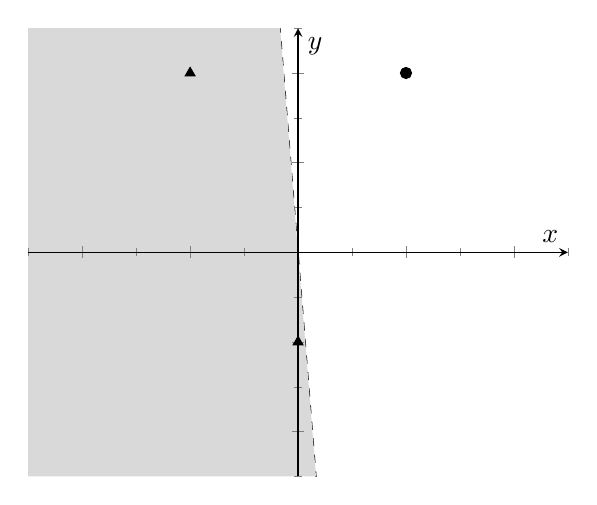
\begin{tikzpicture}
				\begin{axis}[ymin = -2.5, ymax = 2.5, xmax = 2.5, xmin = -2.5, xticklabel = \empty, yticklabel = \empty, minor tick num = 1, axis lines = middle, xlabel = $x$, ylabel = $y$, axis on top]
					\addplot[only marks, mark = *] coordinates {(1, 2)};
					\addplot[only marks, mark = triangle*] coordinates {(-1, 2) (0, -1)};
					\addplot[domain = -3:3, samples = 2, dashed] {-15*x};
					\draw[fill = gray!30, draw = none] (axis cs:-2.5, -2.5) -- (axis cs:-2.5, 2.5) -- (axis cs: -1/6, 2.5) -- (axis cs:1/6, -2.5);
				\end{axis}
			\end{tikzpicture}
			\caption{Puntos separados en $\mathbb{R}^2$}
			\label{fig:separated_label_data}
		\end{figure}
		
		\begin{table}[H]
			\centering
			\begin{tabular}{|c|c|c|}\hline
				$x$ & $y$ & $x \oplus y$\\\hline
				0 & 0 & 0\\\hline
				0 & 1 & 1\\\hline
				1 & 0 & 1\\\hline
				1 & 1 & 0\\\hline
			\end{tabular}
			\caption{Función XOR}
			\label{table:xor}
		\end{table}
		
		\begin{figure}
			\centering
			\begin{tikzpicture}
				\begin{axis}[ymin = -.5, ymax = 2.5, xmax = 2.5, xmin = -.5, xticklabel = \empty, yticklabel = \empty, minor tick num = 1, axis lines = middle, xlabel = $x$, ylabel = $y$]
					\addplot[only marks, mark = *] coordinates {(0, 0) (1, 1)};
					\addplot[only marks, mark = triangle*] coordinates {(0, 1) (1, 0)};
				\end{axis}
			\end{tikzpicture}
			\caption{Valores de $x \oplus y$ en  $\mathbb{R}^2$}
			\label{fig:xor}
		\end{figure}
		
		En cuanto a la pregunta de cómo hallar los parámetros, se consideran las siguientes ecuaciones\cite{nndesign}, donde $\textbf{w}$ es el vector de pesos, $t$ el valor esperado, y $a$ la salida del perceptrón y se aplica el \Cref{algo:perceptron} para obtener los parámetros óptimos. En dicho algoritmo se supondrá que existe una matriz $X$ de $n$ filas que contiene los diferentes $\textbf{x}$. 
		
		\begin{equation}
			\label{eq:perceptron}
			\begin{gathered}
				\textbf{w}(k+1) = \textbf{w}(k) + e(k)\textbf{x}(k)\\
				b(k+1) = b(k) + e(k)\\
				e(k) = t(k) - a(k)\\
				a(k) = \mathcal{U}(\textbf{w}^t(k)\textbf{x}(k))
			\end{gathered}
		\end{equation}
		
		
		\begin{algorithm}
			\SetProgSty{texttt}\DontPrintSemicolon
			
			\caption{Regla de aprendizaje del perceptrón}
			\label{algo:perceptron}
			
			\Datos{$X, \textbf{t}$}
			\Resultado{$\textbf{w}, b$}
			$b \gets 0$\\
			$\textbf{w} \gets$ \texttt{random}\\
			$k \gets 0$\\
			\Repetir{$\lnot$\texttt{acabar}}{
				\texttt{acabar} $\gets$ \texttt{true}\\
				\Para{$i \gets k$ \KwTo $k + n - 1$}{
					$e(i) \gets t(i) - a(i)$\\
					$\textbf{w}(i+1) \gets \textbf{w}(i) + e(i)\textbf{x}(i \pmod n)$\\
					$b(i+1) \gets b(i) + e(i)$\\
					\texttt{acabar} $\gets$ \texttt{acabar} $\land \, e(i) == 0$ 
				}
				$k \gets k + n - 1$
			}
		\end{algorithm}
		
		A cada una de las iteraciones que realiza el bucle exterior se les denomina épocas o \textit{epoch}, que consiste en realizar el proceso de entrenamiento sobre todo el conjunto de datos. En este caso se está suponiendo que no va a recibir casos que no sean linealmente separables, pero de lo contrario se puede añadir un contador \texttt{max\_epochs} y fijar un número máximo para no caer en un bucle infinito. No sería tarea fácil determinar dicho valor, pues aunque el algoritmo converge en los casos previamente explicados, no en todos lo hace de manera rápida. A continuación se muestra cómo obtener una solución para el caso de la \Cref{fig:labeled_data} aplicando el \Cref{algo:perceptron}. 
		
		$$
		X = \begin{pmatrix}
			1 & -1 & 0\\
			2 & 2 & -1
		\end{pmatrix} \,\,\, \textbf{t} = \begin{pmatrix}
		1 & 0 & 0
		\end{pmatrix} \,\,\, \textbf{w}(0) = \begin{pmatrix}
		1\\1 \end{pmatrix} \,\,\, b(0) = 0
		$$
		
		\begin{enumerate}[label = \textbf{\arabic*. }]
			\setcounter{enumi}{-1}
			\item \begin{itemize}
				\item $a(0) = \mathcal{U}(\textbf{w}^t(0)\textbf{x}(0)) = \mathcal{U}\left(\begin{pmatrix}1 & 1\end{pmatrix}\begin{pmatrix}
					1\\2 \end{pmatrix} + 0\right) = 1$
				\item $e(0) = t(0) - a(0) = 1 - 1 = 0$
				\item $\textbf{w}(1) = \textbf{w}(0)$
				\item $b(1) = b(0)$
			\end{itemize}
			
			\item \begin{itemize}
				\item $a(1) = \mathcal{U}(\textbf{w}^t(1)\textbf{x}(1)) = \mathcal{U}\left(\begin{pmatrix}1 & 1\end{pmatrix}\begin{pmatrix}
					-1\\2 \end{pmatrix} + 0\right) = 1$
				\item $e(1) = t(1) - a(1) = 0 - 1 = -1$
				\item $\textbf{w}(2) = \textbf{w}(1) + e(1)\textbf{x}(1) = \begin{pmatrix}1\\ 1\end{pmatrix} - \begin{pmatrix}-1\\2\end{pmatrix} = \begin{pmatrix}2\\ -1\end{pmatrix}$
				\item $b(2) = b(1) + e(1) = -1$
			\end{itemize}
			
			\item \begin{itemize}
				\item $a(2) = \mathcal{U}(\textbf{w}^t(2)\textbf{x}(2)) = \mathcal{U}\left(\begin{pmatrix}2 & -1\end{pmatrix}\begin{pmatrix}
					0\\-1 \end{pmatrix} -1\right) = 1$
				\item $e(2) = t(2) - a(2) = 0 - 1 = -1$
				\item $\textbf{w}(3) = \textbf{w}(2) + e(2)\textbf{x}(2) = \begin{pmatrix}2\\ -1\end{pmatrix} - \begin{pmatrix}0\\-1\end{pmatrix} = \begin{pmatrix}2\\ 0\end{pmatrix}$
				\item $b(3) = b(2) + e(2) = -2$
				\item $\texttt{acabar} = \texttt{true} \land \texttt{false} \land \texttt{false} = \texttt{false}$
			\end{itemize}
			
			\item \begin{itemize}
				\item $a(3) = \mathcal{U}(\textbf{w}^t(3)\textbf{x}(3\pmod{3})) = \mathcal{U}\left(\begin{pmatrix}2 & 0\end{pmatrix}\begin{pmatrix}
					1\\2 \end{pmatrix} -2\right) = 1$
				\item $e(3) = t(3) - a(3) = 1 - 1 = 0$
				\item $\textbf{w}(4) = \textbf{w}(3)$
				\item $b(4) = b(3)$
			\end{itemize}
			
			\item \begin{itemize}
				\item $a(4) = \mathcal{U}(\textbf{w}^t(4)\textbf{x}(4\pmod{3})) = \mathcal{U}\left(\begin{pmatrix}2 & 0\end{pmatrix}\begin{pmatrix}
					-1\\2 \end{pmatrix} -2\right) = 0$
				\item $e(4) = t(4) - a(4) = 0 - 0 = 0$
				\item $\textbf{w}(5) = \textbf{w}(4)$
				\item $b(5) = b(4)$
			\end{itemize}
			
			\item \begin{itemize}
				\item $a(5) = \mathcal{U}(\textbf{w}^t(5)\textbf{x}(5\pmod{3})) = \mathcal{U}\left(\begin{pmatrix}2 & 0\end{pmatrix}\begin{pmatrix}
					0\\-1 \end{pmatrix} -2\right) = 0$
				\item $e(5) = t(5) - a(5) = 0 - 0 = 0$
				\item $\textbf{w}(6) = \textbf{w}(5)$
				\item $b(6) = b(5)$
				\item $\texttt{acabar} = \texttt{true} \land \texttt{true} \land \texttt{true} = \texttt{true}$
			\end{itemize}
		\end{enumerate}
		
		La ejecución del algoritmo finaliza tras dos épocas, donde en la primera de ellas va ajustando los pesos y el sesgo de manera adecuada, y en la segunda verifica que todas las observaciones han sido clasificadas de manera correcta. La frontera de decisión obtenida es la recta $r: 2x - 2 = 0$, que es una recta vertical. Una observación a realizar es que $\textbf{x}(1) \in r$, por tanto ¿a qué clase pertenece? Esto depende de la función de activación empleada, al utilizar $\mathcal{U}$ la clasificación es correcta, pero al cambiarla por otra, podría no serlo y necesitaría de más épocas para realizar correctamente la clasificación. \\
		
		La última cuestión que queda por tratar respecto al perceptrón es el porqué se verifica que en el caso de que los puntos dados sean linealmente separables, en un número finito de pasos, el \Cref{algo:perceptron} terminará su ejecución y con el $\textbf{w}$ óptimo, tal y como se enunciaba en el \textbf{Teorema de Convergencia del Perceptrón}. A continuación se realiza su demostración basándose en la que se encuentra en \cite{nndesign} pero de forma más clara y simple. Para comenzar con la demostración será necesario definir una serie de elementos, comenzando por $\Omega(k)$ y $\textbf{z}(k)$. Se entiende que se están concatenando vectores, no definiendo ``vectores dentro de vectores''. 
		
		$$
		\Omega(k) = \begin{pmatrix}
			\textbf{w}(k)\\
			b(k)
		\end{pmatrix} \,\,\, \textbf{z}(k) = \begin{pmatrix}
		\textbf{x}(k)\\
		1
		\end{pmatrix}
		 \,\,\, \Omega(0) = \begin{pmatrix}
			0\\0\\\vdots\\0
		\end{pmatrix}
		$$
		
		Con estos elementos y el cálculo de $a(k)$ en la \Cref{eq:perceptron} es fácil ver que $n(k) = \Omega^t(k)\textbf{z}(k)$. Recordando los posibles valores de $t(k)$, se deseaba que si dicho valor era 1, entonces $n(k) \geq 0$; y en caso de que valiese 0 entonces se deseaba tener $n(k) < 0$, en resumen, que $t(k) - a(k) = 0$. Otra forma de ver esto es afirmar que en el caso en que $t(k) \neq a(k)$, entonces $\Omega(k)$ debe actualizarse de acuerdo a la \Cref{eq:perceptron}. De esta forma $\Omega(k + 1) = \Omega(k) + e(k)\textbf{z}(k)$. Ahora se considerará un vector $\Omega^*$ de forma que 
		$$
		\forall k \exists \Omega^* \,\, \mathcal{U}(\Omega^{*^t}\textbf{z}(k)) = t(k),
		$$
		es decir, $\Omega^*$ es el vector de pesos óptimo. Además, por comodidad se normalizarán todas las distancias del problema, de manera que $\|\Omega^{*}\| = 1$ y $\|\textbf{z}(k)\| \leq 1$. El último elemento a considerar será $\delta$, que será definido como
		$$
		\delta = \min\lbrace\Omega^{*^t}\textbf{z}(i)\rbrace, 
		$$
		tomando además que $\delta > 0$ pues otra manera de definirlo es la distancia al punto más cercano a la frontera de decisión óptima. Con estos elementos se puede comenzar la demostración. Como la regla de actualización es $\Omega(k + 1) = \Omega(k) + e(k)\textbf{z}(k)$, al vector de pesos en un determinado instante (clasificación fallida) se le suma o resta $\textbf{z}(k)$ y a priori no se sabe cuántas veces se va a repetir esto, por lo que la idea de la demostración será ver si la norma del vector de pesos tiene una cota superior e inferior, es decir, se para de sumar o restar otros vectores $\textbf{z}(i)$, de manera que el algoritmo terminaría. Para obtener esto basta con comparar el comportamiento de $\Omega^t(k) \Omega^*$ frente a $\Omega^t(k)\Omega(k)$ (es decir, $\|\Omega\|^2$). \\
		
		Con el primero de los términos, al tratar de corregir un error se verifica que
		
		$$
		\Omega^t(k+1)\Omega^* = (\Omega(k) + e(k)\textbf{z}(k))^t \Omega^* = \Omega^t(k)\Omega^* + e(k)\Omega^{*^t}\textbf{z}(k). 
		$$
		
		Además, por la manera en la que se ha definido $\delta$, el segundo sumando pertenece al intervalo $(-\infty, -\delta] \cup [\delta, \infty)$, pudiendo deducir la siguiente desigualdad, por lo que en una actualización el término sólo varía por lo menos en $\delta$ unidades.  
		
		\begin{equation}
			\label{eq:inf_delta}
			\Omega^t(k+1)\Omega^* \geq \Omega^t(k)\Omega^* + \delta
		\end{equation}
		
		De la misma manera que se ha analizado el comportamiento de $\Omega^t(k) \Omega^*$ se procede con la actualización de $\Omega^t(k)\Omega(k)$. 
		
		\begin{align*}
			\Omega^t(k+1)\Omega(k+1) &= (\Omega(k) + e(k)\textbf{z}(k))^t(\Omega(k) + e(k)\textbf{z}(k))\\
			&= \Omega^2(k) + (e(k)\textbf{z}(k))^2 + 2e(k)\Omega^t(k)\textbf{z}(k)\\
			&= \Omega^t(k)\Omega(k) + e^2(k)\textbf{z}^t(k)\textbf{z}(k) + 2e(k)\Omega^t(k)\textbf{z}(k)\\
			&= \Omega^t(k)\Omega(k) + e^2(k)\textbf{z}^t(k)\textbf{z}(k) + 2e(k)n(k)
		\end{align*}
		
		En el segundo sumando se tiene que siempre será menor o igual que 1, pues por definición $0 \leq \textbf{z}^t(k)\textbf{z}(k) = \|\textbf{z}(k)\|^2 \leq 1$. Además, el tercer sumando siempre será cero o negativo, pues en todos los casos posibles en los que $e(k) \neq 0$ se cumple que $e(k)n(k) < 0$: 
		
		\begin{itemize}
			\item Si $t(k) = 1 \land n(k) < 0$, entonces $a(k) = 0 \land e(k) > 0$
			\item Si $t(k) = 0 \land n(k) \geq 0$, entonces $a(k) = 1 \land e(k) < 0$
		\end{itemize}
		
		De esta situación se puede deducir la siguiente desigualdad, por lo que en una actualización el término sólo varía en como máximo una unidad.   
		
		\begin{equation}
			\label{eq:sup_delta}
			\Omega^t(k+1)\Omega(k+1) \leq \Omega^t(k)\Omega(k) + 1
		\end{equation}
		
		Una vez se ha observado cómo varían estos términos al actualizarlos, se puede observar qué pasaría con ellos al hacer $m$ actualizaciones. Con el resultado obtenido en las \Cref{eq:inf_delta,eq:sup_delta} se pueden deducir las desigualdades $\delta m \leq \Omega^t(m)\Omega^*$ y $\Omega^t(m)\Omega(m) \leq m$. \\
		
		Ahora al aplicar la desigualdad de Cauchy--Schwarz\footnote{Esta desigualdad afirma que $\|\textbf{u}\textbf{v}\| \leq \|\textbf{u}\|\|\textbf{v}\|$. }, el valor de $\|\Omega^*\|$, y la propiedad transitiva, se obtiene una cota superior y otra inferior (ambas recuadradas) para $\|\Omega^t(m)\|$, lo que demuestra que el número de actualizaciones es finito y que por tanto el algoritmo converge. 
		
		\begin{align*}
			\boxed{\delta m} &\leq \Omega^t(m)\Omega^* = \|\Omega^t(m)\Omega^*\|\\
			&\leq \|\Omega^t(m)\| \|\Omega^*\| = \|\Omega^t(m)\| = \sqrt{\Omega^t(m)\Omega(m)}\\
			& \leq \boxed{\sqrt{m}} 
		\end{align*}
		
		$$
		\pushQED{\qed} 
		\delta m \leq \|\Omega(m)\| \leq \sqrt{m} \,\,\, \Longrightarrow \,\,\, m \leq \frac{1}{\delta^2}\qedhere
		\popQED
		$$ 
		
		Esta última desigualdad muestra cómo existe una relación entre el número de iteraciones del algoritmo y la distancia de los datos de entrenamiento a la frontera de decisión óptima (depende únicamente de esto). Cuanto más cerca estén, mayor será el número de iteraciones necesarias. 
		
	\section{Redes neuronales artificiales}
	
		El descubrimiento del perceptrón junto con el teorema que garantizaba que cualquier conjunto de puntos linealmente separable podría ser aprendido mediante este, supuso un gran avance en la IA al igual que una gran desilusión por parte de muchos al no poder aprender una función tan simple como la XOR. Esto causó el llamado el primer invierno de la IA, que finalizó con la llegada de las redes neuronales multicapa y el algoritmo de la retroprogragación. \\
		
		En 1989, George Cybenko enunció y consiguió demostrar el \textbf{Teorema de Aproximación Universal}\cite{teoremaAproximacion}. Este afirma que dada una red neuronal con una capa de entrada, una capa oculta con suficientes neuronas, y una capa de salida; es un aproximador universal de funciones. Es decir, si existe una relación entre dos variables $\textbf{x}$ e $\textbf{y}$, entonces una red neuronal con la arquitectura mencionada y el entrenamiento adecuado, encontrará dicha relación y podrá comportarse como una función $f$ tal que $\textbf{y} = f(\textbf{x})$. Este se considera un gran resultado, pues consigue acabar con las limitaciones del perceptrón que habían generado un decaimiento por el interés en la IA. 
		
		\begin{figure}[!h]
			\centering
			\begin{tikzpicture}
				\node[circle, draw, fill=gray!20] (x-1) {$x_{1}$};
				\foreach \i in {2,3}{
					\pgfmathtruncatemacro{\resta}{\i - 1}
					\node[circle, draw, fill=gray!20, below = of x-\resta] (x-\i) {$x_{\i}$};
				}
				\node (dots) [below = of x-3] {$\vdots$};
				\foreach \i in {1,2,3}{
					\node[circle, draw, fill=gray!20, right = 2cm of x-\i] (a-\i) {$a^{(1)}_{\i}$};
				}
				\node (dots2) [below = of a-3] {$\vdots$};
				\node (a-4) [circle, draw, fill=gray!20, below = of dots2] {$a^{(1)}_i$};
				\foreach \i in {1,2,3}{
					\node[circle, draw, fill=gray!20, right = 2cm of a-\i] (A-\i) {$a^{(M)}_{\i}$};
				}
				\node (dots3) [below = of A-3] {$\vdots$};
				\node (x-4) [circle, draw, fill=gray!20, left = 2cm of a-4] {$x_n$};
				\node (A-4) [circle, draw, fill=gray!20, below = of dots3] {$a^{(M)}_j$};
				\foreach \i in {1,2,3,4}{
					\node [left = .6cm of A-\i] {$\cdots$};
					\foreach \j in {1,2,3,4}{
						\draw[-] (x-\i) -- (a-\j);
					}
				}
				\foreach \i in {1,2,3}{
					\node (y-\i) [circle, draw, fill=gray!20, right =  of A-\i] {$y_{\i}$};
					\draw[-] (A-\i) -- (y-\i);
				}
				\node (y-4) [circle, draw, fill=gray!20, right =  of A-4] {$y_{j}$};
				\draw[-] (A-4) -- (y-4);
				\node (dots4) [right = 1.6cm of dots3] {$\vdots$};
			\end{tikzpicture}
			\caption{Arquitectura de una red neuronal multicapa}
			\label{fig:rna}
		\end{figure}
		
		En la \Cref{fig:rna} se muestra un diagrama que resume la arquitectura de una red neuronal multicapa. Todas las salidas de una capa están conectadas con todas las entradas de la siguiente con un peso y un \textit{bias}. En el diagrama de la \Cref{fig:rna_completa} se puede observar esto en mayor detalle. Estas pueden ser utilizadas en problemas de clasificación o regresión supervisada, pero en una primera aproximación se supondrá que se está resolviendo un problema de regresión. \\
		
		\begin{figure}
			\centering
			\resizebox{\textwidth}{!}{
				\begin{tikzpicture}
					\node[circle, draw, fill=gray!20] at (4, 0) (n-1) {$n^{(1)}_{1}$};
					\node[circle, draw, fill=gray!20, below= .5cm of n-1] (b-1) {$b^{(1)}_{1}$};
					\foreach \i in {2,3}{
						\pgfmathtruncatemacro{\resta}{\i - 1}
						\node[circle, draw, fill=gray!20, below= 2 cm of b-\resta] (n-\i) {$n^{(1)}_{\i}$};
						\node[circle, draw, fill=gray!20, below= .5cm of n-\i] (b-\i) {$b^{(1)}_{\i}$};
					}
					\node[circle, draw, fill=gray!20, below left = 2 cm and 7 cm of n-1] (x-1) {$x_{1}$};
					\foreach \i in {2,3}{
						\pgfmathtruncatemacro{\resta}{\i - 1}
						\node[circle, draw, fill=gray!20, below= 2cm of x-\resta] (x-\i) {$x_{\i}$};
					}
					\node (dots) [below = .5cm of x-3] {$\vdots$};
					\node[circle, draw, fill=gray!20, below = .5cm of dots] (x-n) {$x_{n}$};
					\node (dots2) [below = .5cm of b-3] {$\vdots$};
					\node[circle, draw, fill=gray!20, below= .5cm of dots2] (n-n) {$n^{(1)}_{i}$};
					\node[circle, draw, fill=gray!20, below= .5cm of n-n] (b-n) {$b^{(1)}_{i}$};
					\foreach \i in {1,2,3}{
						\draw[-] (n-\i) -- (b-\i) node [midway, right] {$1$};
					}
					\draw[-] (b-n) -- (n-n) node [midway, right] {$1$};
					\foreach \i in {1,2,3}{
						\foreach \j in {1,2,3}{
							\pgfmathtruncatemacro{\condicion}{ifthenelse(Mod(\i, 2)==0,1,0)}
							\ifnum\condicion=1
							\draw[-] (x-\i) -- (n-\j) node [near start, above, sloped] {$w^{(1)}_{\j\i}$};
							\else
							\draw[-] (x-\i) -- (n-\j) node [near end, above, sloped] {$w^{(1)}_{\j\i}$};
							\fi
						}
					}
					\foreach \i in {1,2,3}{
						\draw[-] (x-n) -- (n-\i) node [near start, above, sloped] {$w^{(1)}_{\i n}$};
						\draw[-] (x-\i) -- (n-n) node [near end, below, sloped] {$w^{(1)}_{i\i}$};
					}
					\draw[-] (x-n) -- (n-n) node [midway, below, sloped] {$w^{(1)}_{in}$};
					\foreach \i in {1,2,3}{
						\node[circle, draw, fill=gray!20, right = 1cm of n-\i] (a-\i) {$a^{(1)}_{\i}$};
					}
					\node[circle, draw, fill=gray!20, right = 1cm of n-n] (a-n) {$a^{(1)}_{i}$};
					\foreach \i in {1,2,3}{
						\draw[-] (n-\i) -- (a-\i);
					}
					\draw[-] (n-n) -- (a-n);
					\foreach \i in {1,2,3}{
						\node [right = .7cm of a-\i] {$\cdots$};
						\node[circle, draw, fill=gray!20, right = 2cm of a-\i] (N-\i) {$n^{(M)}_{\i}$};
					}
					\node[circle, draw, fill=gray!20, right = 2cm of a-n] (N-4) {$n^{(M)}_{j}$};
					\node [right = .7cm of a-n] {$\cdots$};
					\foreach \i in {1,2,3}{
						\node[circle, draw, fill=gray!20, right = 1cm of N-\i] (A-\i) {$a^{(M)}_{\i}$};
					}
					\node[circle, draw, fill=gray!20, right = 1cm of N-4] (A-4) {$a^{(M)}_{j}$};
					\foreach \i in {1,2,3,4}{
						\draw[-] (N-\i) -- (A-\i);
					}
					\foreach \i in {1,2,3}{
						\node[circle, draw, fill=gray!20, below= .5cm of N-\i] (B-\i) {$b^{(M)}_{\i}$};
						\draw[-] (N-\i) -- (B-\i) node [midway, right] {$1$};
					}
					\node [below = .5cm of B-3] {$\vdots$};
					\node[circle, draw, fill=gray!20, below= .5cm of N-4] (B-4) {$b^{(M)}_{j}$};
					\draw[-] (N-4) -- (B-4) node [midway, right] {$1$};
					\foreach \i in {1,2,3}{
						\node[circle, draw, fill=gray!20, right = 22 cm of x-\i] (y-\i) {$y_{\i}$};
					}
					\node[circle, draw, fill=gray!20, right = 22 cm of x-n] (y-4) {$y_{j}$};
					\foreach \i in {1,2,3,4}{
						\draw[-] (A-\i) -- (y-\i);
					}
				\end{tikzpicture}
			}
			\caption{Red neuronal multicapa}
			\label{fig:rna_completa}
		\end{figure}
		
		Al igual que un perceptrón quedaba representado mediante un vector $\textbf{w}$ de pesos y un valor de sesgo $b$, para representar una red neuronal multicapa se hace mediante las matrices $W^{(m)}$ y los vectores $\textbf{b}^{(m)}$ y $\textbf{f}^{(m)}$, que contienen los pesos, los sesgos, y las funciones de activación. La notación para los sesgos es $b_i^{(m)}$, que representa el sesgo de la entrada $i-$ésima de la capa $m$. De igual manera $f_i^{(m)}$ representa la función de activación la neuona $i-$ésima de la capa $m$. Para los pesos, $w_{ij}^{(m)}$ denota el peso que une la salida $j$ con la entrada $i$ de la capa $m$. Para las capas, $1 \leq m < M$. En ningún momento un exponente entre paréntesis representa una potencia, en dicho caso aparecerá sin paréntesis para distinguirlo. Siguiendo los mismos pasos que con el perceptrón, la primera pregunta será cómo calcular la salida de una red neuronal. La salida de una capa se calcula con la \Cref{eq:prop}, teniendo en cuenta que $\textbf{x}^{(m)} = \textbf{y}^{(m-1)}$, por lo que para calcular la salida de la red no hay más que aplicar dicha ecuación hasta llegar a la última capa. 
		
		\begin{equation}
			\label{eq:prop}
			\begin{gathered}
				\textbf{a}^{(m)}(k) = \textbf{f}^{(m)}\left(W^{(m)}(k)\textbf{x}^{(m)}(k) + \textbf{b}^{(m)}(k)\right)\\
				\begin{pmatrix}
					a_1^{(m)}(k)\\a_2^{(m)}(k)\\\vdots\\a_j^{(m)}(k)
				\end{pmatrix} = \textbf{f}^{(m)}\left(
				\begin{pmatrix}
					w_{11}^{(m)}(k) & w_{12}^{(m)}(k) & \cdots & w_{1i}^{(m)}(k)\\
					w_{21}^{(m)}(k) & w_{22}^{(m)}(k) & \cdots & w_{2i}^{(m)}(k)\\
					\vdots & \vdots & \ddots & \vdots\\
					w_{j1}^{(m)}(k) & w_{j2}^{(m)}(k) & \cdots & w_{ji}^{(m)}(k)\\
				\end{pmatrix}
				\begin{pmatrix}
					x_1^{(m)}(k)\\x_2^{(m)}(k)\\\vdots\\x_i^{(m)}(k)
				\end{pmatrix} + 
				\begin{pmatrix}
					b_1^{(m)}(k)\\b_2^{(m)}(k)\\\vdots\\b_j^{(m)}(k)
				\end{pmatrix}\right)
			\end{gathered}
		\end{equation}
		
		A continuación, se puede plantear cuál es la ecuación del error para una red neuronal. Esta es simplemente cuestión de elección al igual que las funciones de activación. Al trabajar con redes neuronales para problemas de regresión, la función de error por excelencia es el error cuadrático, definido como
		$$
		L(k) = \sum(\textbf{t}(k) - \textbf{a}^{(M)}(k))^2, 
		$$
		aunque existen otras muchas, cada una adecuada a cada tipo de problema y modelo, como por ejemplo el error cuadrático medio, error absoluto, error absoluto medio, error logarítmico, error exponencial, entropía cruzada, etc\cite{funcionesError}.\\
		
		La pregunta ahora sería que, al igual que existía una ecuación para actualizar los parámetros del perceptrón ¿existe para una red neuronal? Para deducirla fácilmente, basta en pensar que $L$ es una función que depende de los parámetros de la red y que se quiere que su valor sea lo más pequeño posible para diferentes vectores de entrada, es decir, encontrar los valores de los parámetros que minimizan $L$. Esto es un problema clásico de cálculo que en el caso de una variable se resuelve igualando a cero la derivada de la función, y en el caso de varias, mediante la matriz Hessiana. Sin embargo, dichos métodos para una función de tantas variables y con expresiones complejas, no son muy eficientes. \\
		
		Esto se soluciona con ayuda de un algoritmo conocido como descenso por gradiente\cite{descenso}. Este algoritmo calcula de manera iterativa una aproximación de los mínimos de una función con ayuda del vector gradiente de una función. El vector gradiente de una función $f$ se define como 
		$$
		\nabla f(x_1, x_2, \hdots, x_n) = \left(\frac{\partial f}{\partial x_1}, \frac{\partial f}{\partial x_2}, \hdots, \frac{\partial f}{\partial x_n}\right), 
		$$
		e indica la dirección en la que la función crece más rápido, siendo la idea principal del algoritmo ir moviéndose en dirección contraria a este. 
		
		\begin{algorithm}
			\SetProgSty{texttt}\DontPrintSemicolon
			
			\caption{Descenso por gradiente}
			\label{algo:descenso}
			
			\Datos{$f, \alpha, k$}
			\Resultado{$\textbf{x}(k)$}
			$\textbf{x}(0) \gets$\texttt{ random}\\
			\Para{$i \gets 1$ \KwTo $k$}{
				$\textbf{x}(i + 1) = \textbf{x}(i) - \alpha\nabla f(\textbf{x}(i))$
			}
		\end{algorithm}
		
		Como se observa en el \Cref{algo:descenso}, se comienza en un punto aleatorio, lo que puede variar la calidad de la solución dependiendo de la ejecución, y además se introduce un término $\alpha$ llamado \textbf{tasa de aprendizaje}. Pueden existir casos en los que la magnitud del gradiente sea muy grande, lo que resulta en desplazamientos bruscos y una convergencia más lenta, tal y como se refleja en la \Cref{fig:descenso}. Si se hubiese fijado un valor máximo de $k = 25$, en los casos de las \Cref{fig:descenso_grande,fig:descenso_peq}, no se hubiese llegado a una buena aproximación del mínimo por haber elegido un $\alpha$ inadecuado. 
		
		\begin{figure}[H]
			\centering
			\begin{subfigure}{.3\textwidth}
				\centering
				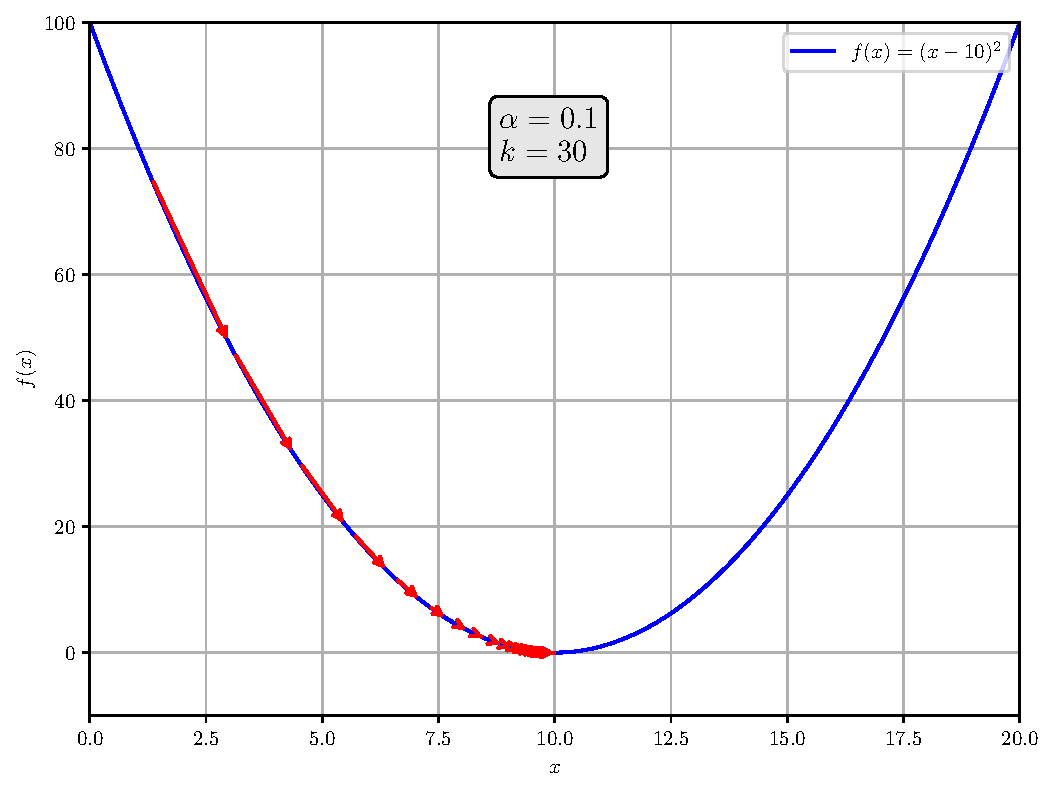
\includegraphics[width = \linewidth]{descenso}
				\caption{$\alpha$ adecuada}
			\end{subfigure}
			\begin{subfigure}{.3\textwidth}
				\centering
				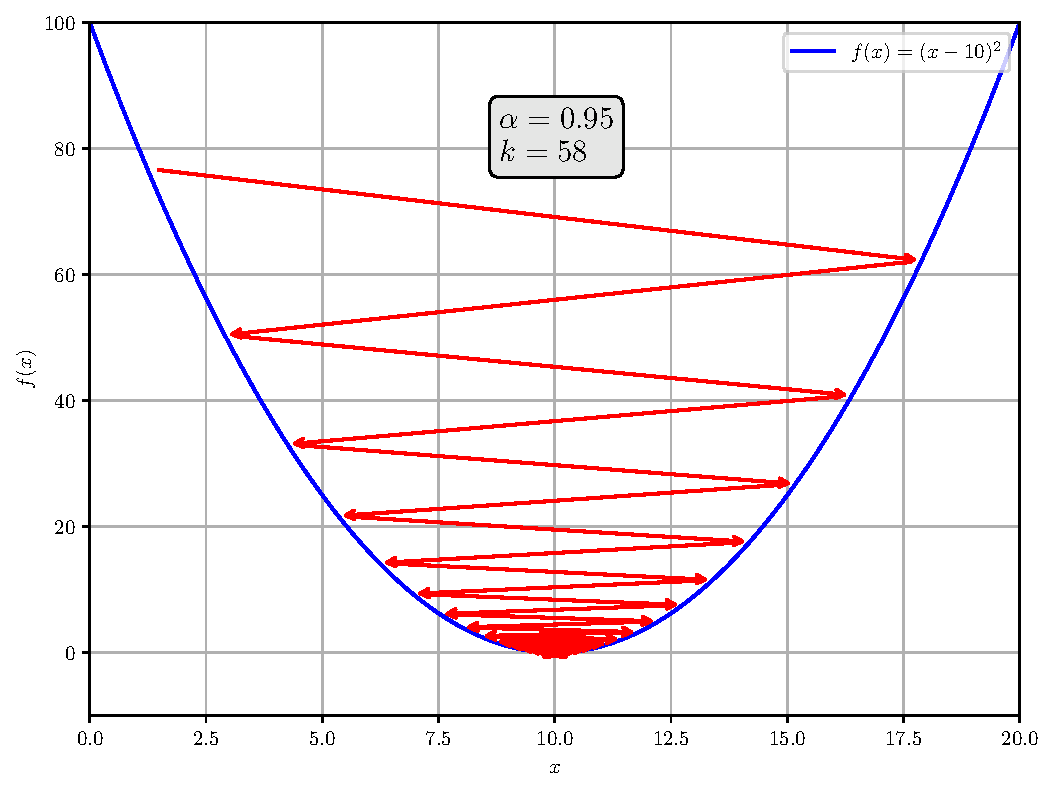
\includegraphics[width = \linewidth]{descenso2}
				\caption{$\alpha$ demasiado grande}
				\label{fig:descenso_grande}
			\end{subfigure}
			\begin{subfigure}{.3\textwidth}
				\centering
				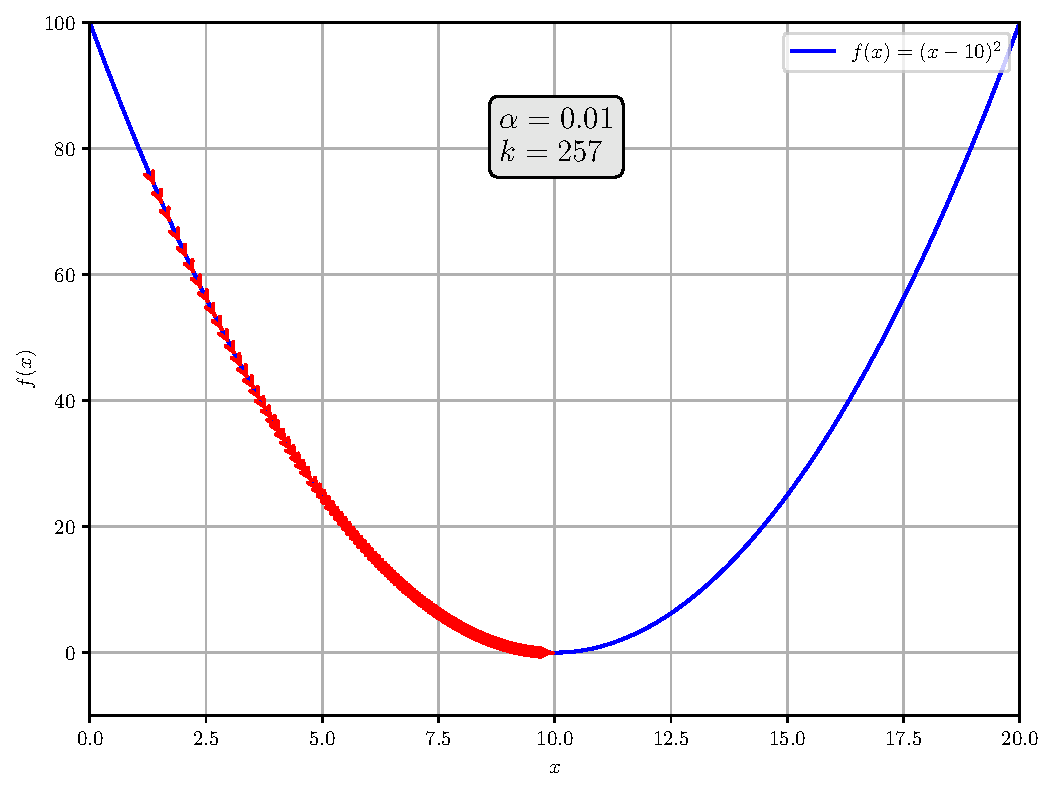
\includegraphics[width = \linewidth]{descenso3}
				\caption{$\alpha$ demasiado pequeña}
				\label{fig:descenso_peq}
			\end{subfigure}
			\caption{Descenso por gradiente}
			\label{fig:descenso}
		\end{figure}
		
		Con esta idea de la función de error y el descenso por gradiente, aparece el famoso algoritmo de la retropropagación o \textit{backpropagation}. Es muy similar al algoritmo de aprendizaje del perceptrón pero adaptado a la estructura de una red neuronal. El primer paso consiste en dada una entrada, calcular la salida de la red con ayuda de la \Cref{eq:prop}. El segundo paso es calcular el error $L(k)$. Esta función depende de todos los pesos y sesgos de la red, por lo que el tercer paso será modificar estos de acuerdo a $\nabla L$ y repetir el procedimiento para el resto de observaciones. Se realizan tantas épocas como sean necesarias. \\
		
		El problema que queda por resolver es cómo calcular todos los elementos de $\nabla L$, pues por ejemplo es fácil calcular $\frac{\partial L}{\partial a_i^{(M)}}$, pero no parece tan obvio calcular $\frac{\partial L}{\partial w_{ij}^{(m)}}$, pues hay que retroceder $M-m$ capas, y habrá muchos valores que dependan de ese peso. La solución a esto es la regla de la cadena. 
		
		$$
		\frac{\partial f}{\partial x} = \sum_{i=1}^n \frac{\partial f}{\partial u_{i1}}\frac{\partial u_{im}}{\partial x}\prod_{j=1}^{m-1}\frac{\partial u_{ij}}{\partial u_{ij+1}}
		$$
		
		Con ayuda de esta regla se pueden calcular fácilmente los términos no triviales del gradiente, propagando el error hacia atrás por la red hasta llegar al parámetro deseado mediante las sensibilidades $\left(\delta_i^{(s)}\right)$\cite{nndesign}. De aquí se intuye el porqué del nombre del algoritmo. De manera informal, lo que hace el algoritmo es castigar a cada neurona de manera proporcional a su participación en el error final. 
		
		$$
		\begin{gathered}
			\frac{\partial L}{\partial b_{i}^{(s)}} = \frac{\partial L}{\partial a_{i}^{(s)}} \frac{\partial a_{i}^{(s)}}{\partial n_{i}^{(s)}} \frac{\partial n_{i}^{(s)}}{\partial b_{i}^{(s)}} = \delta_i^{(s)}\\
			\frac{\partial L}{\partial w_{ij}^{(s)}} = \frac{\partial L}{\partial a_{i}^{(s)}} \frac{\partial a_{i}^{(s)}}{\partial n_{i}^{(s)}} \frac{\partial n_{i}^{(s)}}{\partial w_{ij}^{(s)}} = \delta_i^{(s)} \frac{\partial n_{i}^{(s)}}{\partial w_{ij}^{(s)}} = \delta_i^{(s)} a_j^{(s-1)}\\
			\delta_i^{(M)} = \frac{\partial L}{\partial a_{i}^{(M)}} \frac{\partial a_{i}^{(M)}}{\partial n_{i}^{(M)}} = -2a_{i}^{(M)} \frac{\partial a_{i}^{(M)}}{\partial n_{i}^{(M)}} = -2a_{i}^{(M)} \frac{\partial f_{i}^{(M)}}{\partial n_{i}^{(M)}}\\
			\delta_i^{(m)} = \frac{\partial L}{\partial n_i^{(m)}} = \sum_{l=1}^p\frac{\partial L}{\partial n_l^{(m+1)}}\frac{\partial n_l^{(m+1)}}{\partial n_i^{(m)}} = \sum_{l=1}^p \delta_l^{(m+1)} \frac{\partial n_l^{(m+1)}}{\partial n_i^{(m)}} = \sum_{l=1}^p \delta_l^{(m+1)} w_{li}^{(m+1)} \frac{\partial f_i^{(m)}}{\partial n_i^{(m)}}\\
			\text{con } 0 < m < M \text{ y } 0 < s \leq M
		\end{gathered}
		$$
		
		Estas ecuaciones pueden reescribirse de manera matricial para aligerar la notación, que combinándolas con las ideas explicadas referentes al \Cref{algo:descenso}, da lugar al \Cref{algo:backprop}, bastante similar al \Cref{algo:perceptron} pero adaptado a una red neuronal. \\
		
		\begin{algorithm}
			\SetProgSty{text}\DontPrintSemicolon
			
			\caption{Retropropagación (\textit{backpropagation})}
			\label{algo:backprop}
			
			\Datos{$\textbf{f}^{(s)}, \textbf{x}^{(1)}(k), \textbf{t}(k), \varepsilon$}
			\Resultado{$W^{(s)}, \textbf{b}^{(s)}$}
			
			\Para{$i \gets 1$ \KwTo $\varepsilon$}{
				\ParaCada{$\textbf{x}^{(1)}$}{
					\texttt{calcular} $\textbf{a}^{(M)}(k)$\\
					\texttt{calcular} $L(k)$ y $\nabla L(k)$\\
					$
					\begin{gathered}
						\delta^{(M)}(k) \gets -2 \frac{\partial \textbf{f}^{(M)}}{\partial \textbf{n}^{(M)}}(\textbf{t}(k) - \textbf{a}^{(M)}(k))\\
						\delta^{(m)}(k) \gets \frac{\partial \textbf{f}^{(M)}}{\partial \textbf{n}^{(M)}} W^{(m+1)^t}(k)\delta^{(m+1)}(k)
					\end{gathered}
					$\\
					$W^{(m)}(k+1) \gets W^{(m)}(k) - \alpha \delta^{(m)}(k)(\textbf{a}^{(m-1)}(k))^t$\\
					$\textbf{b}^{(m)}(k+1) \gets \textbf{b}^{(m)}(k) - \alpha \delta^{(m)}(k)$
				}
			}
		\end{algorithm}
		
		En esta variante del algoritmo (denominada estocástica o \textbf{SGD}) se actualizan los parámetros por cada observación del \textit{dataset} y se ha decidido elegir como criterio de parada alcanzar un número de épocas, aunque también se suelen tomar otros criterios, como la magnitud del error. Además, esta variante es computacionalmente costosa, pues para cada observación se calcula el gradiente. Otra variante del algoritmo es el \textbf{batch}. Esta no actualiza por cada observación como SGD, halla el gradiente del error promedio de todas las observaciones del \textit{dataset}. No es recomendable, pues es muy costosa y si el \textit{dataset} ocupa mucho, puede no caber en memoria. Ambas aproximaciones se pueden combinar para dar lugar a una variante más eficiente que estas dos, denominada \textbf{mini-batch}, que realiza lo mismo que \textit{batch} pero dividiendo el \textit{dataset} en \textit{minibatches} y realizando una actualización de los parámetros por cada uno de ellos. De esta manera no se necesita tener todo el \textit{dataset} en memoria\cite{descenso}. 
		
		\subsection{Funciones de activación}
		
			Durante el estudio del perceptrón, se muestra cómo se emplea la función de Heaviside como función de activación en la neurona. Esto se debe a que se busca una función que independientemente de los valores de entrada que reciba, produzca una salida binaria. En ciertos casos, no se deseará una salida binaria pues el problema no tendría porqué ser de clasificación, como se ha visto con las redes neuronales. Además, como se ha visto en el \Cref{algo:backprop}, será imprescindible poder calcular la derivada de estas funciones. Por estos motivos, se presentan las funciones de activación más conocidas e importantes\cite{funcionesActivacion}. 
			
			\begin{itemize}
				\item \textbf{Función lineal}
				
				\begin{figure}[!h]
					\centering
					\begin{tikzpicture}
						\draw[->] (-2,0) -- (2,0) node[right] {$x$};
						\draw[->] (0,-2) -- (0,2) node[above] {$f(x)$};
						
						\draw[domain = -2:2, smooth, variable = \x] plot ({\x},{\x});
						\node[right] at (1.5,2.5) {$f(x) = x$};
					\end{tikzpicture}
					\caption{Función lineal}
					\label{fig:funcion_lineal}
				\end{figure}
				
				Con motivo de emplear una función que no produzca valores binarios, se pueden tomar funciones lineales $f: \mathbb{R} \longrightarrow \mathbb{R}$ de la forma $f(x) = ax$. No es muy útil al trabajar con tareas complejas, solo es capaz de cumplir con su tarea en problemas sencillos, y esto en parte se debe a la expresión de su derivada. Al ser un polinomio, es continua y derivable en todo $\mathbb{R}$, teniendo que
				$$
				\frac{df}{dx} = a. 
				$$
				
				\item \textbf{Función logística}
				
				\begin{figure}[!h]
					\centering
					\begin{tikzpicture}
						\begin{axis}[
							xlabel = $x$,
							ylabel = {$f(x)$},
							xmin = -10, xmax = 10,
							ymin = 0, ymax = 1,
							width = 0.8\textwidth,
							height = 0.35\textwidth,
							xticklabel = \empty,
							yticklabel = \empty,
							axis lines = middle,
							domain = -10:10,
							samples = 100,
							]
							\addplot[black] {1/(1 + exp(-x))};
							\node at (axis cs: 5,0.8) {$f(x) = \frac{1}{1 + e^{-x}}$};
						\end{axis}
					\end{tikzpicture}
					\caption{Función logística}
					\label{fig:funcion_sigmoide}
				\end{figure}
				
				Esta también es una función que no devuelve valores binarios, es conocida como función sigmoide por la forma de S que tiene, y es una función $f: \mathbb{R} \longrightarrow (0, 1)$. Una propiedad que es muy útil es que es solución de la ecuación diferencial
				$$
				\frac{df}{dx} = f(x)(1 - f(x)). 
				$$
				
				Es un intento de mejora de la función de activación empleada en el perceptrón, pues una ligera variación en la entrada puede crear un gran cambio en la salida. Esta función evita que eso suceda, pues una pequeña variación en la entrada produce una variación pequeña en la salida. 
				
				\item \textbf{Tangente hiperbólica}
				\begin{figure}[!h]
					\centering
					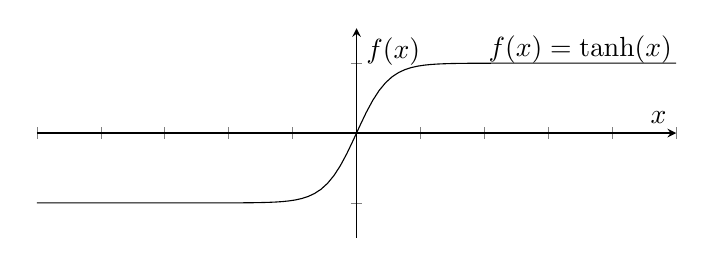
\begin{tikzpicture}
						\begin{axis}[
							xlabel = $x$,
							ylabel = {$f(x)$},
							xmin = -10, xmax = 10,
							ymin = -1.5, ymax = 1.5,
							width = 0.8\textwidth,
							height = 0.35\textwidth,
							xticklabel = \empty,
							yticklabel = \empty,
							axis lines = middle,
							domain = -10:10,
							samples = 100,
							]
							\addplot[black] {tanh(x)};
							\node at (axis cs: 7, 1.2) {$f(x) = \tanh(x)$};
						\end{axis}
					\end{tikzpicture}
					\caption{Tangente hiperbólica}
					\label{fig:funcion_tanh}
				\end{figure}
				
				De nuevo, esta función no devuelve valores binarios, y que guarda cierta relación con la logística, pues esta tiene también forma de sigmoide, pero a diferencia que la logística, esta verifica que $f(-x) = -f(x)$ por lo que es preferible sobre esta, y también hace que al usarla en redes neuronales su entrenamiento converja más rápido. Además $f: \mathbb{R} \longrightarrow (-1, 1)$ y su expresión es
				$$
				f(x) = \tanh(x) = \frac{\text{senh}(x)}{\cosh(x)} = \frac{e^x - e^{-x}}{e^x + e^{-x}}, 
				$$
				y verifica una segunda propiedad muy útil, es solución de la ecuación diferencial
				$$
				\frac{df}{dx} = 1 - f^2(x). 
				$$
				
				\item \textbf{Función ReLU}
				
				\begin{figure}[H]
					\centering
					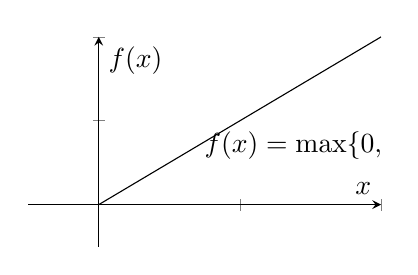
\begin{tikzpicture}
						\begin{axis}[
							xlabel = $x$,
							ylabel = {$f(x)$},
							xmin = -.5, xmax = 2,
							ymin = -.5, ymax = 2,
							width = 0.5\textwidth,
							height = 0.35\textwidth,
							xticklabel = \empty,
							yticklabel = \empty,
							axis lines = middle,
							domain = -.5:2,
							samples = 100,
							]
							\addplot[black, domain = 0:2] {x};
							\node at (axis cs: 1.5, .7) {$f(x) = \max\{0, x\}$};
						\end{axis}
					\end{tikzpicture}
					\caption{Función ReLU}
					\label{fig:funcion_relu}
				\end{figure}
				
				La función ReLU (Rectified Linear Unit) es una de las más populares al trabajar con redes neuronales, pues a pesar de que no es derivable en $x = 0$ (normalmente se soluciona tomando $f'(0) = 1$), soluciona un serio problema que causan las funciones logística y tangente hiperbólica durante el entrenamiento de una red neuronal. Este problema es conocido como \textit{vanishing gradient} y de forma resumida consiste en que cuando la derivada de una función de activación es muy próxima a cero, relentiza enormemente el proceso de aprendizaje, pues si se observa con detalle cómo se calculan las actualizaciones de los pesos y sesgos en el \Cref{algo:backprop}, si los términos $\delta^{(s)}$ tienden a cero, la diferencia entre los parámetros de una iteración a otra tiende a cero, necesitando una cantidad enorme de iteraciones. Como se observa a continuación, la función ReLU soluciona este problema. Además, la derivada es mucho más sencilla de calcular. 
				
				\begin{align*}
					\lim_{x\to\infty}\frac{d}{dx}\frac{1}{1+e^{-x}} = 0 && \lim_{x\to\infty}\frac{d}{dx}\tanh(x) = 0 && \lim_{x\to\infty}\frac{d}{dx}\text{ReLU}(x) = 1
				\end{align*}
				
				Si bien soluciona este problema mencionado para valores de $x > 0$, genera el mismo problema para valores negativos. Para solucionar este problema se suelen tomar variantes de la función ReLU conocidas como LReLU, PReLU, o ELU; que modifican su expresión para valores de $x \leq 0$ como funciones lineales o exponenciales. 
				
			\end{itemize}
			
		\section{Redes neuronales convolucionales}
		
			Una vez explicado cómo funciona una red neuronal y cómo puede usarse para problemas de regresión y clasificación, es interesante poder aplicar estas tareas sobre imágenes en vez de sobre conjuntos de datos numéricos. Una imagen de $n \times m$ píxeles en escala de grises puede entenderse como una matriz de $n \times m$ elementos, sin embargo, suelen utilizarse imágenes a color y esto se puede conseguir utilizando tres canales, rojo, azul, y verde. De esta forma, una imagen se representa como tres matrices. Formalmente, una imagen se representa como un tensor, que puede entenderse como un vector de matrices, o una estructura que indexa elementos mediante una tupla $(i, j, k)$\cite{introCNN}.\\
			
			De manera ingenua, una primera aproximación para clasificar imágenes en función de objetos que aparezcan en estas, podría ser linealizar este tensor y pasarlo como vector de entrada a un red neuronal multicapa, obteniendo un vector de salida que indique a qué clase pertenece la imagen. Esto, además de que no da resultados positivos, pues se da la misma importancia a todos los píxeles y se obvian detalles y características de la imagen, computacionalmente es muy complicado de abarcar. Suponiendo que se tiene una imagen RGB cuadrada de $n \times n$ píxeles, y que la primera capa oculta tuviera $m$ neuronas, el número de parámetros de esta capa sería $m(3n^2 + 1)$. Suponiendo imágenes de baja calidad, por ejemplo $64 \times 64$ píxeles, y que el número de neuronas de la primera capa fuese 5, el número de parámetros es de 61445. Ajustar adecuadamente esa cantidad de parámetros muy costoso, y además daría resultados muy pobres en el caso de encontrar los parámetros adecuados. 
 		
		
	\paginavacia
	\chapter{Optimización del proceso de valoración de puntos de interés}

	Después de analizar diversos modelos de aprendizaje automático, junto con sus características y los algoritmos asociados, se ofrece un ejemplo práctico que ilustra la aplicación de estos modelos para abordar un problema de la vida real y buscar una solución adecuada. Para ello se presenta la compañía Niantic, fundada en 2010 como parte de una startup de Google, que se especializa en el desarrollo de juegos para dispositivos móviles que utilizan realidad aumentada (AR). Algunas de sus creaciones más destacadas han sido los juegos Ingress y Pokémon GO. \\
	
	Una de las herramientas creadas por esta empresa es Niantic Lightship, que permite a desarrolladores Unity integrar realidad aumentada y mapas con puntos de interés basados en la ubicación real del jugador. Dado que para Niantic resultaba inviable marcar dichos puntos de interés alrededor de todo el mundo, creó Niantic Wayfarer. En esta herramienta, usuarios experimentados de sus juegos pueden hacer propuestas de puntos de interés (llamados Wayspots) para que de manera colaborativa, otros usuarios las valoren. Sin embargo, tras varios años desde su lanzamiento, debido al gran número de propuestas y al reducido número de valoradores, la comunidad notifica largos tiempos de espera en el proceso de valoración de las propuestas. Por este motivo, se propone en este proyecto realizar una primera aproximación a la automatización de este proceso mediante las técnicas de visión e inteligencia artificial presentadas en el marco teórico. \\
	
	La valoración de un Wayspot en Wayfarer consta de diferentes etapas. En primer lugar se muestra un título y descripción del Wayspot junto con la imagen que aparecería en los juegos. Además aparece una imagen secundaria con una visión desde otra perspectiva, junto con otro texto que ayudarían al valorador a ubicar la propuesta, tal y como se muestra en la \Cref{fig:info_propuesta}. También aparece un breve cuestionario con una serie de preguntas genéricas que ayudan a determinar si aquello que se solicita cumple una serie de criterios (\Cref{fig:preguntas}). Además, se muestra un mapa que contiene los Wayspots cercanos para verificar que no exista ya, y comprobar con Street View la ubicación sugerida (\Cref{fig:mapa}). Finalmente, se pide clasificar la propuesta en una o varias categorías (\Cref{fig:etiquetas_propuesta}). 
	
	\begin{figure}[!h]
		\centering
		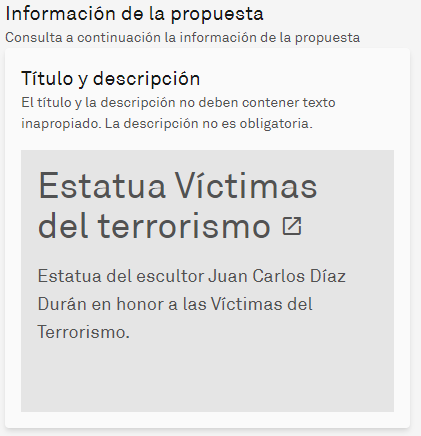
\includegraphics[scale = .4, valign = c]{info_principal}\hfill
		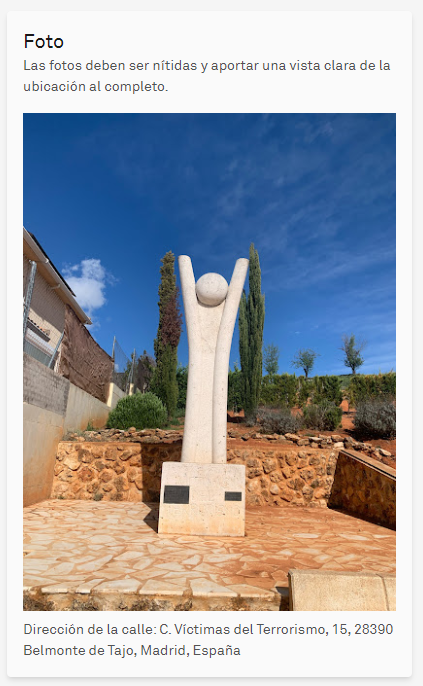
\includegraphics[scale = .4, valign = c]{imagen_principal}\hfill
		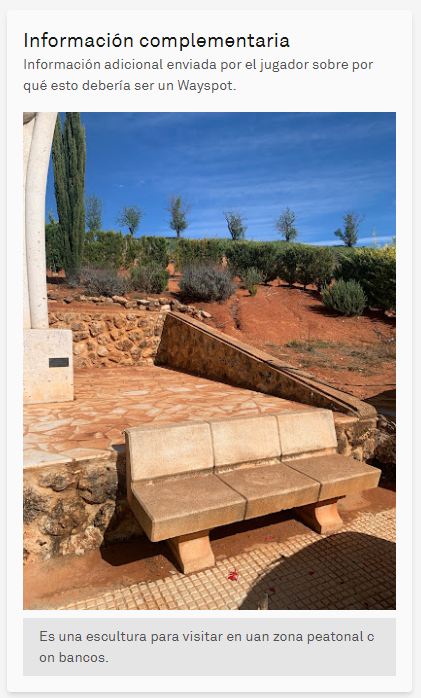
\includegraphics[scale = .4, valign = c]{imagen_secundaria}
		\caption{Información de una propuesta en Wayfarer}
		\label{fig:info_propuesta}
	\end{figure}
	
	\begin{figure}[!h]
		\centering
		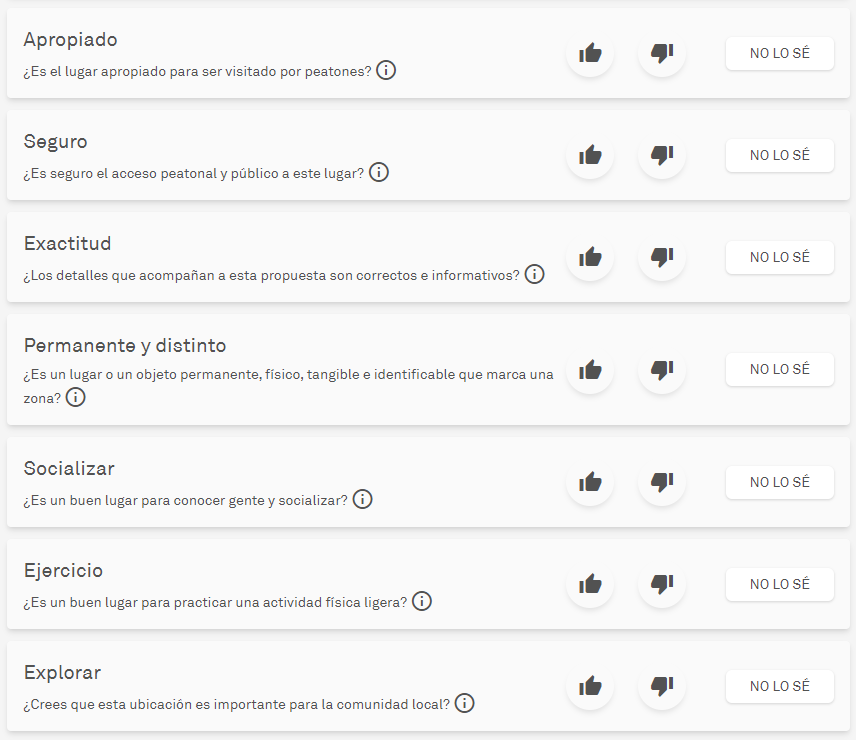
\includegraphics[scale = .4]{cuestionario}
		\caption{Cuestionario de una propuesta en Wayfarer}
		\label{fig:preguntas}
	\end{figure}
	
	\begin{figure}[!h]
		\centering
		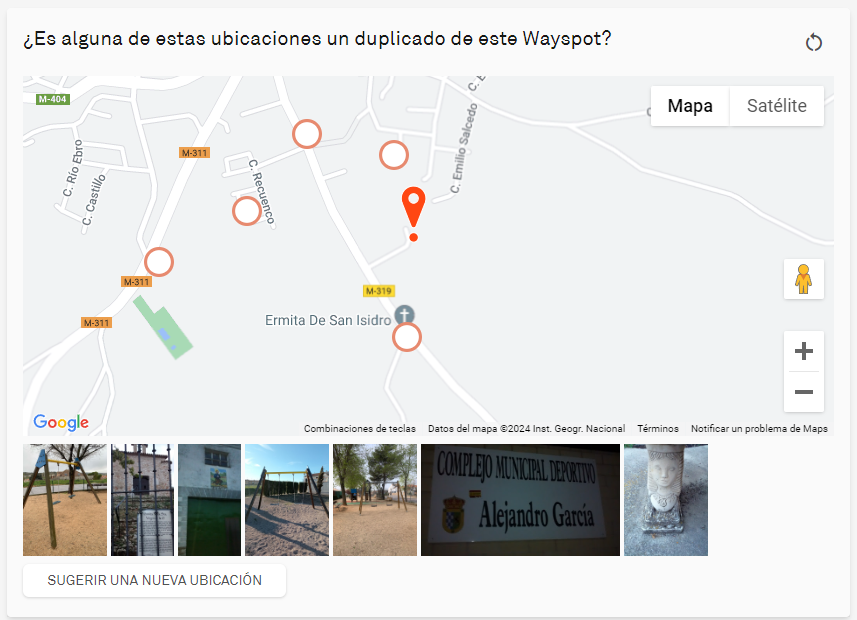
\includegraphics[scale = .4]{mapa}
		\caption{Mapa en una propuesta de Wayfarer}
		\label{fig:mapa}
	\end{figure}
	
	\begin{figure}[!h]
		\centering
		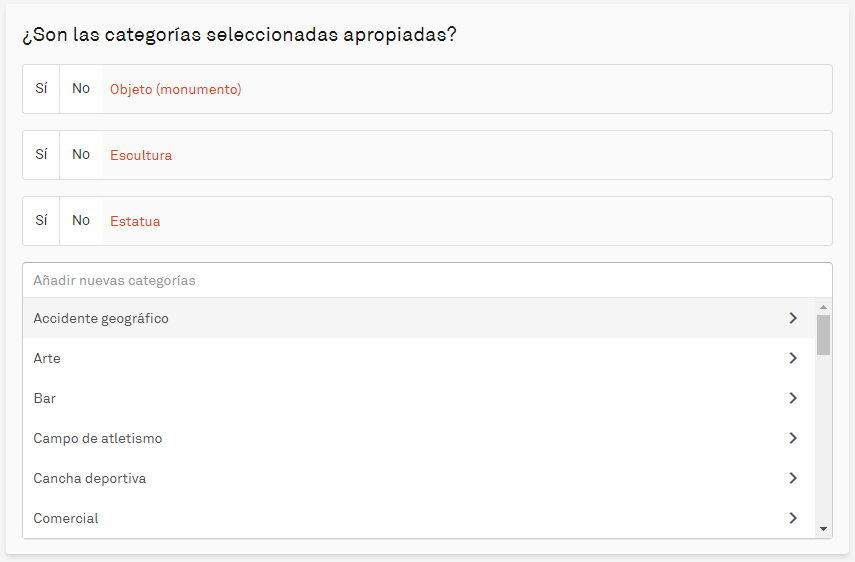
\includegraphics[scale = .4]{etiquetas}
		\caption{Clasificación de una propuesta de Wayfarer}
		\label{fig:etiquetas_propuesta}
	\end{figure}

	\section{Clasificación de imágenes mediante redes convolucionales}
	
		Una primera aproximación a agilizar el proceso de valoración comentado, sería detectar el objeto que se muestra en la imagen de la propuesta, para que en caso de que sea algo aceptable proseguir con el proceso de valoración, o en caso contrario, rechazar directamente la propuesta. En general, en función del objeto que aparezca en la imagen, se tienen directamente las respuestas a las preguntas de la \Cref{fig:preguntas}. \\
		
		Para comenzar este caso práctico, lo primero a realizar es el proceso conocido como ETL, que consiste en la extracción, transformación, y carga de los datos; para posteriormente poder trabajar con ellos y proporcionárselos al modelo. Comenzando por la extracción de datos, se presenta el primero de los problemas. La idea es utilizar imágenes que realmente hayan pasado por este proceso de valoración para poder hacer el proyecto lo más realista posible, sin embargo, ni Wayfarer ni ninguno de los juegos poseen alguna API (al menos de manera pública) que permita recolectar de manera programática las imágenes utilizadas o información relativa a ellas. 
		
		\subsection{Proceso ETL}
		
			La solución adoptada para este proceso, ha sido recolectar manualmente imágenes que han superado el proceso de valoración, pudiendo consultar algunas de ellas desde el mapa de uno de los juegos (\url{https://intel.ingress.com/}). En este caso, se estarían clasificando entre las $n$ clases de objetos aceptables las imágenes recibidas, cosa que en un primer momento parece carecer de sentido pues se conoce el resultado de la valoración. Sin embargo, al no tener acceso a propuestas rechazadas, no se pueden recolectar estos datos para entrenar los modelos, pero si de la empresa responsable se tratase, se dispondría de una enorme cantidad de imágenes válidas y no válidas etiquetadas (gracias a la parte del proceso de valoración que muestra la \Cref{fig:etiquetas_propuesta}), y que se podrían cargar de manera automática. En resumen, cambiando simplemente los datos que se cargarían y su fuente, se podrían tomar las siguientes decisiones sin necesidad de modificar el resto del proyecto.  
			
			\begin{itemize}
				\item Si $I \in C_i, 0 \leq i < m$, rechazar la propuesta
				\item Si $I \in C_j, m \leq j < n$, continuar evaluando la propuesta
			\end{itemize}
			
			Continuando con la extracción de los datos, y preparándolos para la carga, se ha creado una carpeta \texttt{tfg\_dataset} que representa el conjunto de las imágenes que se utilizan durante el proyecto. Dentro de esta, se ubicarán dos subcarpetas, \texttt{train} y \texttt{test}, que hacen referencia a las imágenes que se utilizarán para entrenar los modelos, y las que se utilizarán para evaluar su rendimiento. Para generar dichas carpetas partiendo de una que contiene las imágenes separadas por clases, se ha codificado la función \texttt{split\_tt} que permite hacer la división del conjunto en los de entrenamiento y test con el porcentaje especificado. Previamente a la ejecución de esta función, se recomienza ejecutar otra que se ha codificado llamada \texttt{renombrar\_imagenes}, que dada la ruta raíz donde se encuentran las carpetas de cada clase, renombra las imágenes de cada carpeta de manera que queden enumeradas. Esta es la manera de etiquetar el conjunto de datos y prepararlo para la carga. Se puede visualizar un breve esquema de esta estructura en la \Cref{fig:arbol_dataset}. \\
			
			\begin{figure}[!h]
				\centering
				\scriptsize
				\Tree[.\texttt{tfg\_dataset} [.\texttt{train} [.\texttt{clase\_1} $\vdots$ ] [.\texttt{clase\_2} \texttt{0.jpg} $\cdots$ \texttt{22.jpg} ] $\cdots$ [.\texttt{clase\_n} $\vdots$ ] ] [.\texttt{test} [.\texttt{clase\_1} $\vdots$ ] [.\texttt{clase\_2} \texttt{10.jpg} $\cdots$ \texttt{33.jpg} ]  $\cdots$ [.\texttt{clase\_n} $\vdots$ ] ] ]
				\caption{Árbol de carpetas del dataset}
				\label{fig:arbol_dataset}
			\end{figure}
			
			Para cargar el dataset en TensorFlow directamente desde la estructura de carpetas creadas, se hará uso de la función \texttt{image\_dataset\_from\_directory} de \texttt{utils}. Esta contiene una serie de parámetros interesantes a comentar. 
			
			\begin{itemize}
				\item \texttt{directory}: es el directorio raíz del dataset, en este caso \texttt{tfg\_dataset}. 
				\item \texttt{image\_size}: es una tupla de dos elementos con las dimensiones en píxeles que deberán tener las imágenes del dataset. 
				\item \texttt{labels}: mediante el valor \texttt{inferred} las etiquetas toman el mismo valor que el nombre de las carpetas. 
				\item \texttt{label\_mode}: hace referencia a la forma de codificar las etiquetas. Se empleará el valor \texttt{categorical} para codificar las etiquetas utilizando one-hot-encoding, es decir, si se tienen por ejemplo cuatro clases y un elemento pertenece a la cuarta, dicha etiqueta queda codificada como 0001. 
				\item \texttt{batch\_size}: hace referencia al tamaño de batch o lote que será utilizado durante el entrenamiento. Si en la función de entrenamiento se elige un tamaño diferente, se utilizará el menor de los valores. 
				\item \texttt{validation\_split}: hace referencia al porcentaje de los datos de entrenamiento que se reservan para validar el modelo durante el entrenamiento, es decir, permiten calcular el error del modelo al hacer una predicción de datos que nunca ha visto mientras entrena. Se reservarán un 20\% de los datos para validar. 
				\item \texttt{seed}: hace referencia a la semilla que se utiliza para ordenar las imágenes de manera aleatoria. 
				\item \texttt{subset}: seleccionando el valor \texttt{both} permite devolver el conjunto de entrenamiento y validación con la llamada a la función, es decir, \texttt{x\_train, x\_val = image\_dataset\_from\_directory(...)}. 
			\end{itemize}
			
			Como se puede observar, esta función que está haciendo principalmente el trabajo de la carga de datos, también hace parte del proceso de transformación, ya que permite modificar las dimensiones de la imagen (en este caso se utilizará un valor de $224 \times 224$ píxeles, se justificará más adelante), y también permite modificar la codificación de las etiquetas. Además, cada píxel (en cada canal de color) toma un valor entre 0 y 255. Es muy importante normalizar estos valores en el proceso de transformación para facilitar el trabajo a los diferentes modelos. Para ello, con ayuda de una capa de reescalado de Keras, se divide el valor de cada píxel entre 255 para obtener valores entre 0 y 1. Con motivo de verificar que todos estos pasos se han realizado correctamente, se codificado una función llamada \texttt{sample\_ds\_dfd} que permite visualizar nueve ejemplos aleatorios de un dataset creado con la función de TensorFlow mencionada, obteniendo como resultado la \Cref{fig:sample_dataset}. \\
			
			\begin{figure}
				\centering
				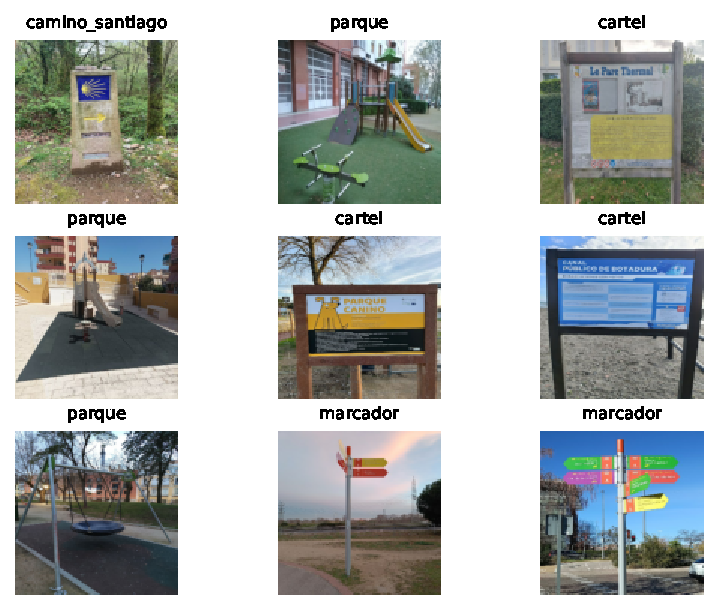
\includegraphics[scale = .8]{sample_dataset}
				\caption{Visualización de ejemplo de un dataset creado}
				\label{fig:sample_dataset}
			\end{figure}
			
		\subsection{Creación y entrenamiento de una red convolucional en TensorFlow}\label{subsec:crear_cnn}
		
			En esta primera aproximación se va a crear y entrenar una red convolucional desde cero con el dataset mencionado. En este caso, se han elegido cuatro tipos de objetos que frecuentemente se proponen como puntos de interés: parques infantiles, carteles informativos, marcadores de ruta, e hitos del Camino de Santiago. Mediante la clase \texttt{Sequential} de Keras, se puede proporcionar una lista de las capas que conforman el modelo. La primera de ellas será una capa de convolución, con la particularidad de que se debe indicar el tamaño de entrada, siendo este un tensor de las dimensiones indicadas en la creación del dataset. Se alterna cada capa de convolución ReLU de stride $3 \times 3$ y 32 o 64 filtros, con una capa de maxpooling con stride $2 \times 2$. Estos valores han sido elegidos de manera arbitraria. Esta arquitectura se puede visualizar en la \Cref{fig:arq_cnn}. \\
			
			\begin{figure}[!h]
				\centering
				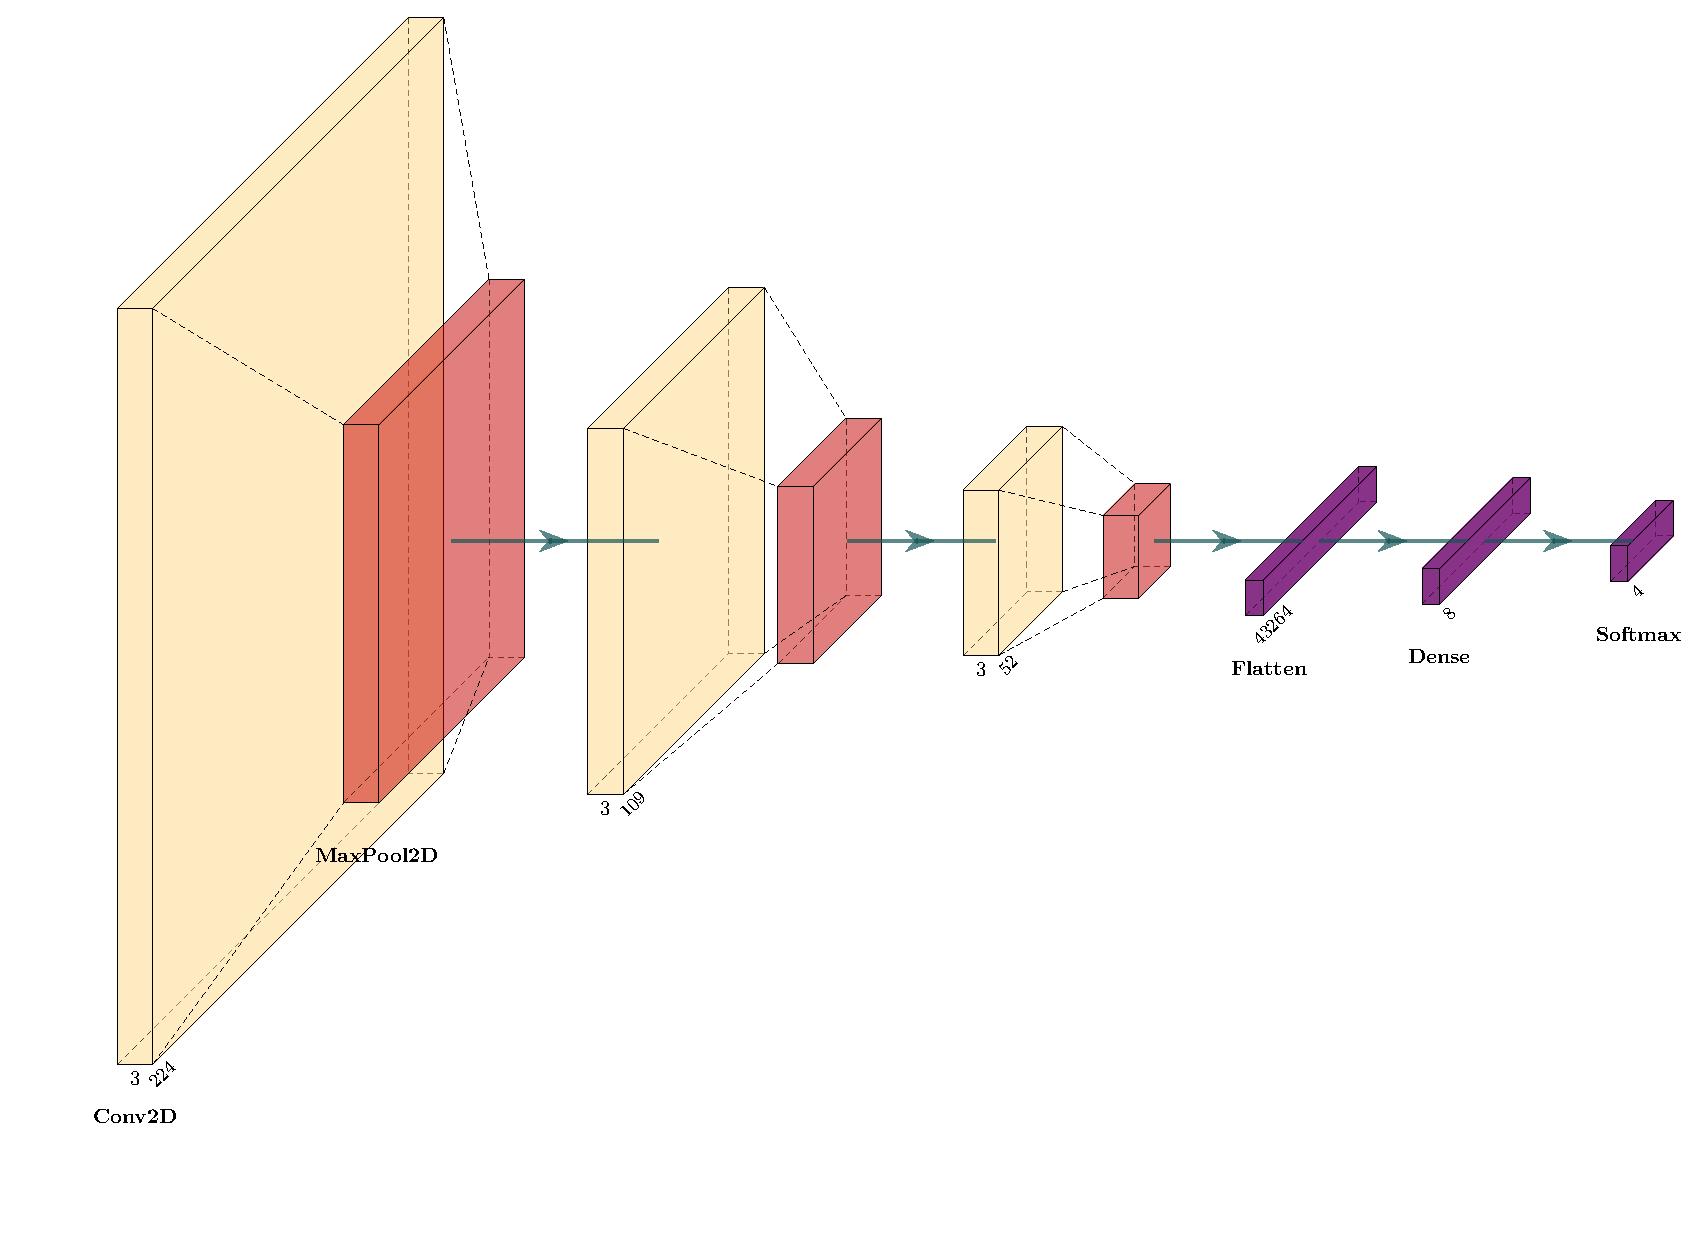
\includegraphics[scale = .55]{arq_cnn}
				\caption{Arquitectura de la red convolucional}
				\label{fig:arq_cnn}
			\end{figure}
			
			Mediante estas capas, se supone que la red debe extraer características de las imágenes, como por ejemplo
			
			\begin{itemize}
				\item Aparece un objeto rectangular
				\item Tiene dos patas 
				\item No tiene formas curvas
			\end{itemize}
			y de ahí con ayuda de una red clásica, ser capaz de deducir que en la imagen aparece un cartel. En realidad, las capas de convolución no obtienen características tan claras, pero sí resultan con una matriz de detalles en la imagen que pueden conducir a la misma conclusión. Para ello se utiliza la capa \texttt{Flatten} que transforma dicha matriz en un vector que sirve de entrada a la siguiente y última capa de la red, una capa oculta con tantas neuronas como clases diferentes. Como función de activación se utiliza softmax para obtener una distribución de probabilidad en la que se observe cuál es claramente la clase a la que pertenece el objeto, y con qué confianza lo es. Finalmente, mediante la función \texttt{summary} se puede observar un resumen del modelo. 
			
			\begin{verbatim}
				_________________________________________________________________
				Layer (type)                Output Shape              Param #   
				=================================================================
				conv2d (Conv2D)             (None, 222, 222, 32)      896       
				
				max_pooling2d (MaxPooling2  (None, 111, 111, 32)      0         
				D)                                                              
				
				conv2d_1 (Conv2D)           (None, 109, 109, 64)      18496     
				
				max_pooling2d_1 (MaxPoolin  (None, 54, 54, 64)        0         
				g2D)                                                            
				
				conv2d_2 (Conv2D)           (None, 52, 52, 64)        36928     
				
				max_pooling2d_2 (MaxPoolin  (None, 26, 26, 64)        0         
				g2D)                                                            
				
				flatten (Flatten)           (None, 43264)             0         
				
				dense_2 (Dense)             (None, 8)                 346120    
				
				dense_3 (Dense)             (None, 4)                 36        
				
				=================================================================
				Total params: 402476 (1.54 MB)
				Trainable params: 402476 (1.54 MB)
				Non-trainable params: 0 (0.00 Byte)
				_________________________________________________________________
			\end{verbatim}
			
			Con la función \texttt{compile} se termina de crear el objeto que representa al modelo, pudiendo especificar un optimizador, la función de pérdida, y las métricas que se muestran durante el entrenamiento. Para este proyecto se utilizarán Adam, entropía cruzada, y precisión respectivamente. El modelo ya está en condiciones de ser entrenado, y esto se logra mediante la función \texttt{fit}, a la que se le proporcionan los datos de entrenamiento (\texttt{x\_train}), los datos de validación (\texttt{x\_val}), el número de épocas (en este caso se han elegido 25), y la ruta de los callbacks. Esta sirve para ir almacenando metadatos del entrenamiento, que mediante una utilidad con la que cuenta TensorFlow llamada TensorBoard, permite monitorizar de manera muy visual la calidad del entrenamiento, tal y como se muestra en la \Cref{fig:tb_cnn}. \\
			
			\begin{figure}[!h]
				\centering
				\begin{subfigure}{.4\textwidth}
					\centering
					\includesvg[width = .85\textwidth]{evaluation_loss_vs_iterations_cnn}
					\caption{Iteraciones frente a pérdida}
					\label{fig:tb_cnn_a}
				\end{subfigure}\hfill
				\begin{subfigure}{.4\textwidth}
					\centering
					\includesvg[width = .85\textwidth]{evaluation_accuracy_vs_iterations_cnn}
					\caption{Iteraciones frente a precisión}
					\label{fig:tb_cnn_b}
				\end{subfigure}
				\begin{subfigure}{.4\textwidth}
					\centering
					\includesvg[width = .85\textwidth]{epoch_loss_cnn}
					\caption{Pérdida sobre el conjunto de entrenamiento y validación}
					\label{fig:tb_cnn_c}
				\end{subfigure}\hfill
				\begin{subfigure}{.4\textwidth}
					\centering
					\includesvg[width = .85\textwidth]{epoch_accuracy_cnn}
					\caption{Precisión sobre el conjunto de entrenamiento y validación}
					\label{fig:tb_cnn_d}
				\end{subfigure}
				\caption{Pérdida y precisión durante el entrenamiento de la CNN}
				\label{fig:tb_cnn}
			\end{figure}
			
			La situación que describen las gráficas, es negativa y sería la típica no deseada, pues se observa como con el paso de las iteraciones el error crece mientras que la precisión se estanca en valores no deseados. En concreto, en la \Cref{fig:tb_cnn_c} se observa cómo el error sobre el conjunto de validación crece, mientras que sobre el conjunto de entrenamiento tiende a cero. Esta es una situación denominada como sobreaprendizaje u \textit{overfitting}\cite{overfitting}. La red no tiene capacidad de aprender ni generalizar, y lo que está haciendo es memorizar los datos de ejemplo que se le presentan, cometiendo entonces errores cuando recibe datos que no ha visto nunca. 
			
		\subsection{Transfer learning en TensorFlow}
		
			Como se ha podido observar durante la sección anterior, el resultado del entrenamiento no ha sido adecuado, pues la red tendía a memorizar los datos que se le presentaban sin mostrar una buena capacidad de generalización. Esto puede deberse a múltiples factores, como por ejemplo, que al tener un conjunto de datos de entrenamiento tan reducido no sea capaz de extraer correctamente las características que determinan a los objetos de cada clase. Es decir, en vez de hacerle llegar a las capas densas hechos como ``tiene un objeto rectangular'', ``tiene dos patas'', etc; podría estar haciéndole llegar, ``hay dos árboles en el fondo''. Observando la estructura del modelo, se está tratando de optimizar cerca un millón de parámetros con poco más de 500 observaciones, algo que es muy desproporcionado; la red no es capaz de encontrar relaciones con tan pocos datos. \\
			
			En proyectos similares del mundo real, y en los que además se dispone de pocos datos (como es el caso), es muy poco frecuente crear y entrenar un modelo desde cero tal y como se ha realizado en la \Cref{subsec:crear_cnn}. En vez de realizar esto, es muy común utilizar una técnica conocida como transfer learning. Tal y como se menciona en \cite{transfer}, es una técnica muy aplicada en casos en los que se dispone de pocos datos y los modelos de deep learning no son capaces de encontrar relaciones, y también en casos en los que se dispone de equipos con pocos recursos. Consiste en aplicar el conocimiento obtenido de otro dataset, no necesariamente relacionado, para facilitar el proceso de obtener el conocimiento deseado del dataset actual. \\
			
			En el problema que se está tratando, se va a aplicar esta técnica de la siguiente manera. Como previamente se ha mencionado, las redes convolucionales, pueden verse como un conjunto de capas capaces de extraer características de las imágenes, junto con una red neuronal clásica que es capaz de clasificar en función de dichas características. Teniendo en cuenta que el principal problema del modelo anterior podría ser que no fuera capaz de obtener las características adecuadas que definen a cada clase, la idea es utilizar una serie de capas que sí sean capaces de obtener de manera correcta las características de una imagen, para después poder entrenar la red neuronal clásica con las características adecuadas. \\
			
			Con ayuda de la librería TensorHub que trabaja junto con TensorFlow, se pueden importar modelos ya entrenados de \url{https://www.kaggle.com/}. En este caso para aplicar la técnica de transfer learning, se ha decidido utilizar la red MobileNet de Google que se observa en la \Cref{fig:mb}. El modelo se puede importar como si de una capa se tratase al crear un modelo secuencial de Keras. Para lograr la técnica, será clave declarar que los parámetros de dicha capa no se deberán entrenar (pues al importar el modelo ya vienen con unos valores adecuados). A continuación se coloca una capa densa, encargada de clasificar las características que la red de Google extraiga, y que deberá ser entrenada. Esta vez, el número de parámetros a optimizar sí es más adecuado al número de observaciones disponibles. 
			
			\begin{figure}[!h]
				\centering
				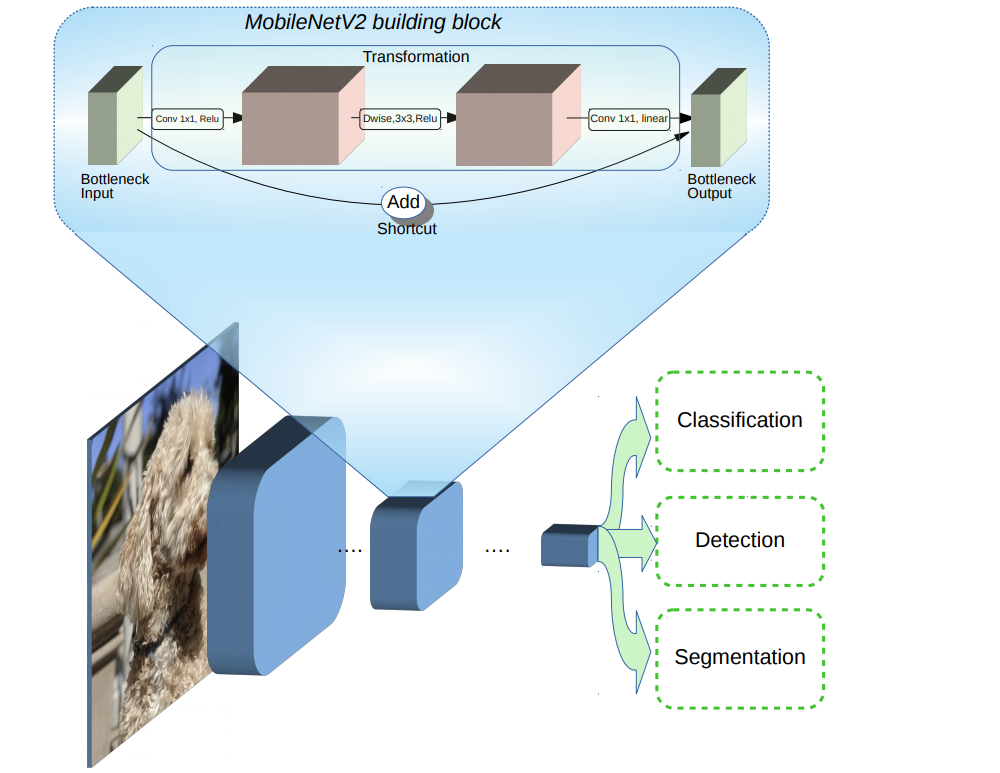
\includegraphics[scale = .3]{mb}
				\caption{MobileNetV2}
				\label{fig:mb}
			\end{figure}
			
			\begin{verbatim}
				_________________________________________________________________
				Layer (type)                Output Shape              Param #   
				=================================================================
				keras_layer (KerasLayer)    (None, 1280)              2257984   
				
				dense (Dense)               (None, 8)                 10248     
				
				dense_1 (Dense)             (None, 4)                 36        
				
				=================================================================
				Total params: 2268268 (8.65 MB)
				Trainable params: 10284 (40.17 KB)
				Non-trainable params: 2257984 (8.61 MB)
				_________________________________________________________________
			\end{verbatim}
			
			La manera de lanzar el entrenamiento es la misma que en el anterior, sin embargo, esta vez los resultados obtenidos son totalmente distintos, tal y como muestran las gráficas de TensorBoard en la \Cref{fig:tb_tl}. \\
			
			\begin{figure}[!h]
				\centering
				\begin{subfigure}{.4\textwidth}
					\centering
					\includesvg[width = .85\textwidth]{evaluation_loss_vs_iterations_mb}
					\caption{Iteraciones frente a pérdida}
					\label{fig:tb_tl_a}
				\end{subfigure}\hfill
				\begin{subfigure}{.4\textwidth}
					\centering
					\includesvg[width = .85\textwidth]{evaluation_accuracy_vs_iterations_mb}
					\caption{Iteraciones frente a precisión}
					\label{fig:tb_tl_b}
				\end{subfigure}
				\begin{subfigure}{.4\textwidth}
					\centering
					\includesvg[width = .85\textwidth]{epoch_loss_mb}
					\caption{Pérdida sobre el conjunto de entrenamiento y validación}
					\label{fig:tb_tl_c}
				\end{subfigure}\hfill
				\begin{subfigure}{.4\textwidth}
					\centering
					\includesvg[width = .85\textwidth]{epoch_accuracy_mb}
					\caption{Precisión sobre el conjunto de entrenamiento y validación}
					\label{fig:tb_tl_d}
				\end{subfigure}
				\caption{Pérdida y precisión durante el entrenamiento aplicando transfer learning}
				\label{fig:tb_tl}
			\end{figure}
			
			Estas gráficas representan una situación cercana a la ideal. En las \Cref{fig:tb_tl_a,fig:tb_tl_b} se observa cómo con el paso de las iteraciones, el error disminuye y la precisión aumenta hasta llegar a valores adecuados. Además, en las \Cref{fig:tb_tl_c,fig:tb_tl_d} se muestra claramente que tanto el error como la precisión se comportan de manera similar sobre los conjuntos de entrenamiento y validación respectivamente, tomando además valores adecuados. 
			
		\subsection{Aumento de datos}
		
			Como se ha visto a lo largo de las secciones anteriores, uno de los problemas que se está teniendo en este caso práctico, es la falta de datos. Una técnica utilizada frecuentemente en estos casos es conocida como aumento de datos. Consiste en modificar las imágenes del dataset de entrenamiento para que el modelo disponga de más ejemplos diferentes\cite{augm}. Podría entenderse como una parte del proceso de transformación ETL. \\
			
			Una vez más, es posible aplicar esta técnica mediante funciones de TensorFlow. Para ello se crea un objeto de la clase \texttt{ImageDataGenerator}. Mediante su constructor se pueden declarar los valores que toman los atributos que modificarán las imágenes, siendo algunos de los más destacables: 
			
			\begin{itemize}
				\item \texttt{rotation\_range}: gira la imagen. 
				\item \texttt{width\_shift\_range} y \texttt{height\_shift\_range}: desplazamiento horizontal y vertical de la imagen. 
				\item \texttt{shear\_range}: estira la imagen. 
				\item \texttt{zoom\_range}: hace zoom a la imagen. 
				\item \texttt{reescale}: indica el factor por el que se reescala la imagen, en este caso $1/255$ para facilitar el entrenamiento a la red, como en casos anteriores. 
				\item \texttt{validation\_split}: porcentaje de los datos reservados a validación. 
			\end{itemize}
			
			Una vez se tiene declarado el generador, se utiliza su método \texttt{flow\_from\_directory} para que dada la ruta que contiene las imágenes, el tamaño deseado de imagen, y el tamaño de los lotes, se cree el objeto que representa al dataset. De manera similar a la anterior, se ha programado una función \texttt{sample\_ds\_ffd} que permite visualizar nueve elementos del dataset creado, tal y como muestra la \Cref{fig:sample_dataset_au}. Esta es una de la manera más común de crear datos nuevos, siendo alguna de las más novedosas las arquitecturas GAN. Están formadas por dos redes, una capaz de crear imágenes y otra capaz de distinguir entre imágenes reales y generadas, y transmitir dicho conocimiento a la primera red, de manera que una intente ``engañar'' a la otra\cite{gan}. \\
			
			\begin{figure}
				\centering
				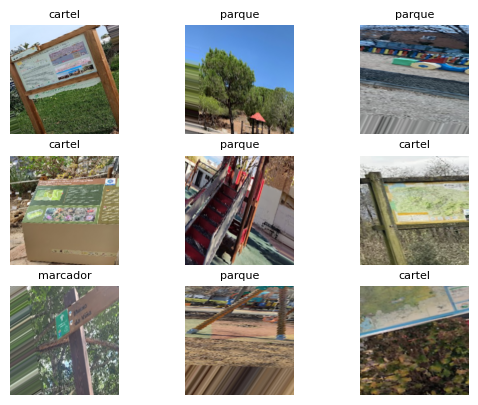
\includegraphics[scale = .8]{sample_dataset_au}
				\caption{Visualización de ejemplo de un dataset aplicando aumento de datos}
				\label{fig:sample_dataset_au}
			\end{figure}
			
			Contando ahora con el dataset original y el modificado, la técnica del aumento de datos se puede aplicar de dos formas. La primera de ellas es crear un modelo y entrenar únicamente con el datset modificado. Esto puede dar una mayor capacidad de generalización al modelo al mostrar imágenes más diferentes de objetos similares. La segunda de ellas consiste en entrenar el modelo con el dataset original, y después con el dataset modificado (sin cambiar qué imágenes pertenecen a los conjuntos de entrenamiento, validación, y test en cada dataset). Esta puede dar mejores resultados, pues tiene más observaciones y el modelo puede de ver el mismo objeto ``de diferentes formas''. Sin embargo hay que tener cuidado con esta segunda opción, pues podría conducir a situaciones de sobreajuste. 
			
		\subsection{Evaluación de los modelos}
		
			Si bien gracias a las gráficas que TensorBoard proporciona es posible hacerse una idea de la calidad que tendrán las predicciones de un modelo, no son suficientes. Será entonces el momento de presentar al modelo una serie de imágenes que nunca haya visto para poder evaluar la calidad de sus predicciones mediante una serie de métricas y valores estadísticos. Este conjunto de imágenes que el modelo no ha recibido hasta el momento, es el denominado conjunto de test. \\
			
			Para calcular estas métricas en Python, se va a utilizar la librería Scikit-learn, ya que contiene un conjunto de métodos con los que calcular y visualizar la mayoría de métricas empleadas en machine learning. Además, las predicciones sobre los conjuntos de test quedará representadas mediante dos matrices, \texttt{Y\_matrix} y \texttt{Y\_score}. La primera de ellas es una matriz $n \times 3$ que contiene para cada observación su etiqueta real, la predicha, y con qué probabilidad se le asigna. La segunda, contiene las probabilidades de cada observación de pertenecer a cada clase, por tanto es de dimensiones $n \times c$. 
			
			\begin{align*}
				Y_m &= \begin{pmatrix}
					0 & 0 & 0.75\\
					2 & 2 & 0.7\\
					3 & 1 & 0.97\\
					\vdots & \vdots & \vdots\\
					1 & 1 & 0.87
				\end{pmatrix} & 
				Y_s &= \begin{pmatrix}
					0.75 & 0.07 & 0.01 & 0.17\\
					0.15 & 0.01 & 0.7 & 0.14\\
					0.02 & 0.97 & 0.01 & 0.01\\
					\vdots & \vdots & \vdots & \vdots\\
					0.05 & 0.87 & 0.01 & 0.08
				\end{pmatrix}
			\end{align*}
			
			Dependiendo si el problema en cuestión es de regresión o clasificación, se deben utilizar unas métricas u otras. Debido a que se desea evaluar la calidad de una clasificación, se han elegido las siguientes. 
			
			\subsubsection{Matriz de confusión}
			
				La matriz de confusión muestra en el caso de clasificación binaria, los verdaderos positivos, verdaderos negativos, falsos positivos, y falsos negativos, mientras que en el caso de clasificación no binaria, en general la relación entre las etiquetas reales de cada observación y las que el modelo le ha asignado\cite{confusion}. De manera muy visual se puede observar la cantidad de ejemplos de cada clase (pudiendo ver si se encuentran desbalanceadas), cuántos han sido clasificados correctamente, cuántos no, y en general entre qué clases suele confundirse más el modelo. \\
				
				\begin{figure}[!h]
					\centering
					\begin{subfigure}{.4\textwidth}
						\centering
						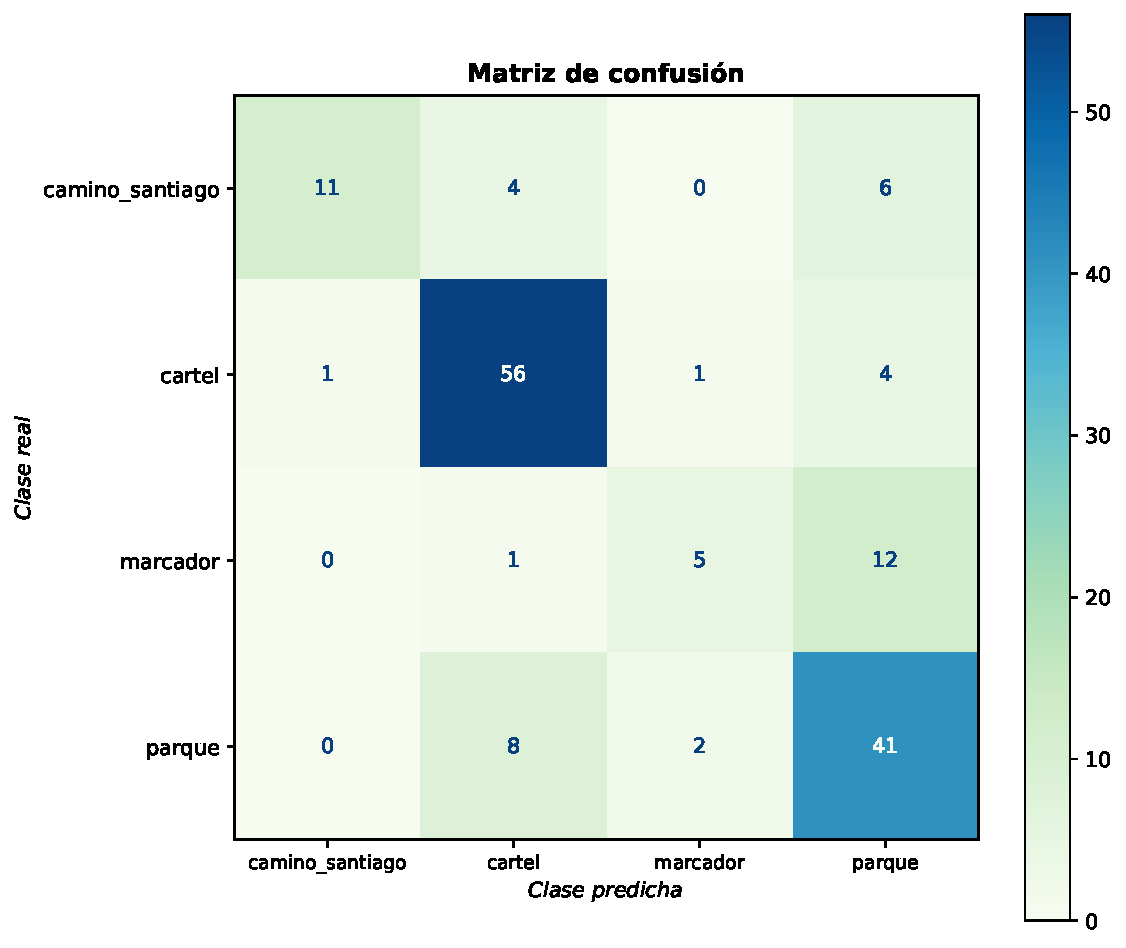
\includegraphics[scale = .42]{mc_conv}
						\caption{Normal}
						\label{fig:mc_conv}
					\end{subfigure}\hfill
					\begin{subfigure}{.4\textwidth}
						\centering
						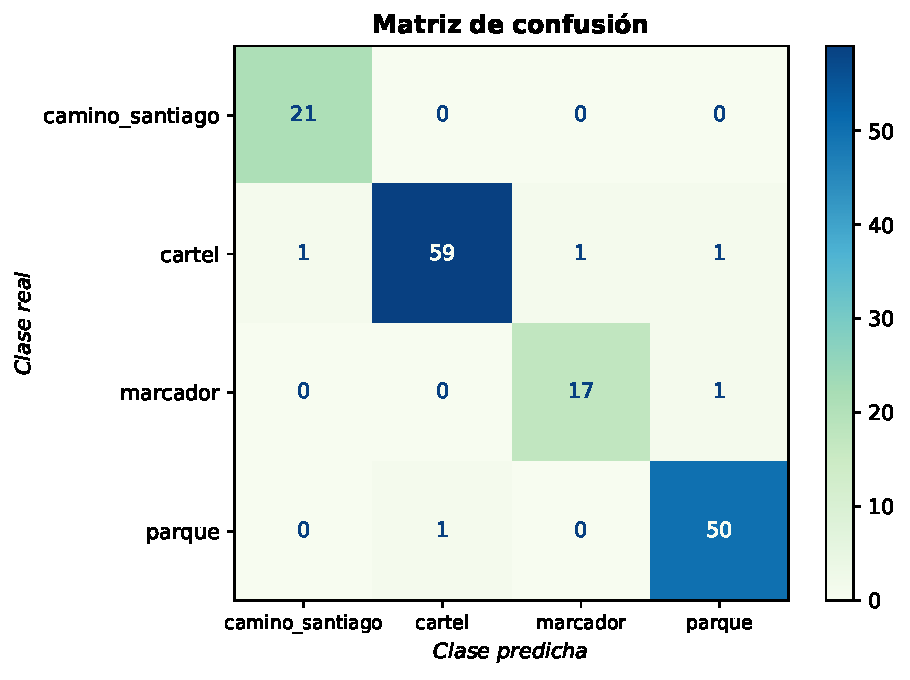
\includegraphics[scale = .42]{mc_mb}
						\caption{Aplicando transfer learning}
						\label{fig:mc_mb}
					\end{subfigure}
					\begin{subfigure}{.4\textwidth}
						\centering
						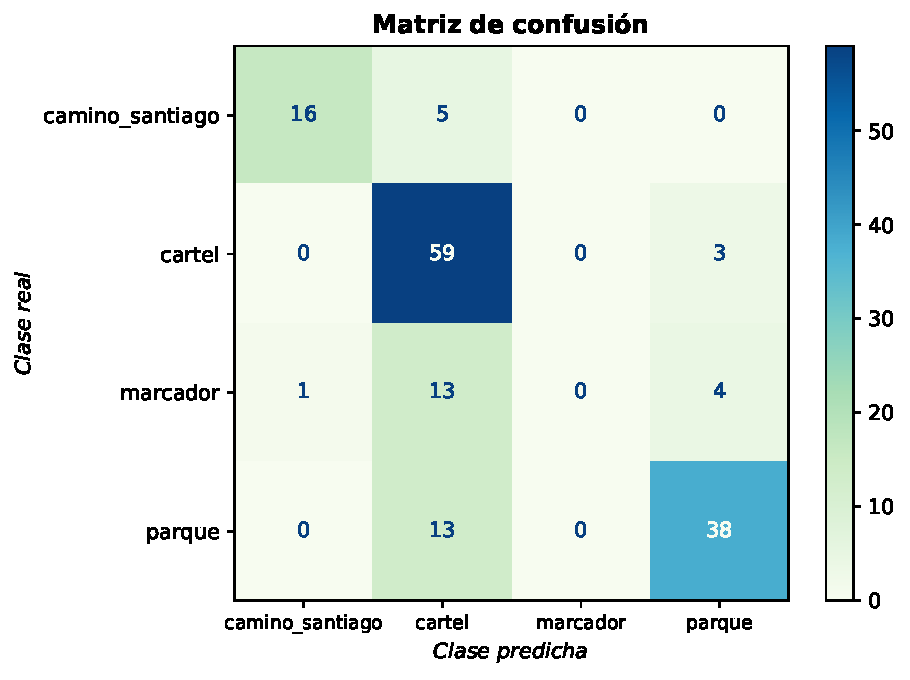
\includegraphics[scale = .42]{mc_convau}
						\caption{Aplicando aumento de datos}
						\label{fig:mc_convau}
					\end{subfigure}\hfill
					\begin{subfigure}{.4\textwidth}
						\centering
						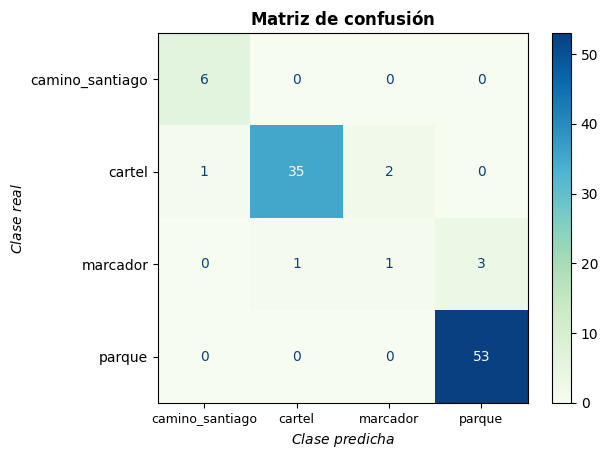
\includegraphics[scale = .42]{mc_mbau}
						\caption{Aplicando ambas}
						\label{fig:mc_mbau}
					\end{subfigure}
					\caption{Matrices de confusión}
					\label{fig:mc}
				\end{figure}
				
				En la \Cref{fig:mc} se observan las matrices de confusión de las cuatro situaciones descritas anteriormente. El elemento $a_{ij}$ representa la cantidad de observaciones de la clase $C_i$ que han sido clasificadas como $C_j$ (a partir de ahora, $\hat{C}_j$). La situación ideal se da cuando en el caso de que $i \neq j$, entonces $a_{ij} = 0$, o lo que es lo mismo, que solo haya valores  en la diagonal principal, pues a todos se les estaría asignando la clase correcta. Además, en esta representación gráfica sería deseable que todos los elementos de dicha diagonal tuviesen el mismo color, pues la situación actual describe un desbalanceo entre las clases. Se ve claramente que al aplicar transfer learning (\Cref{fig:mc_mb,fig:mc_mbau}) se obtienen resultados mucho mejores que al entrenar el modelo desde cero, tal y como las curvas de TensorBoard parecían indicar, pues la cantidad de malas clasificaciones es muy pequeña. La diferencia en dicho caso entre usar aumento de datos o no, no es muy significativa. \\
				
				Para poder calcular la matriz de confusión, se ha utilizado la función \texttt{confusion\_matrix} de Scikit-learn, que recibe como parámetros un vector con las clases reales de cada observación, y otro con las que el modelo les ha asignado. Mediante la función \texttt{ConfusionMatrixDisplay} se puede ver de manera gráfica la matriz (\Cref{fig:mc}). Con diferentes parámetros se pueden cambiar los colores e incrustar código \LaTeX{} para modificar los textos. Se ha codificado la función \texttt{matriz\_confusion} que recibe el dataset y $Y_m$, y muestra el gráfico con la configuración personalizada. 
				
			\subsubsection{Precisión, sensibilidad, y $F_1-$score}
				
				Si bien la matriz de confusión permite mostrar de manera visual la calidad de las clasificaciones, es conveniente calcular algunos valores \cite{metricas_matriz} a partir de esta matriz que permitan visualizar de manera numérica dichas calidades. La primera de ellas conocida como \textbf{precisión} $(\mathcal{P})$, y puede entenderse como la probabilidad de que un elemento que etiquetado como $C_i$, realmente pertenezca a dicha clase. 
				
				$$
				\mathcal{P} = P(C_i | \hat{C}_i) = \frac{P(C_i \cap \hat{C}_i)}{P(\hat{C}_i)}
				$$
				
				La siguiente se denomina \textbf{sensibilidad} (o recuerdo, $\mathcal{R}$) e indica la probabilidad de que un elemento de la clase $C_i$, se clasifique como tal. 
				
				$$
				\mathcal{R} = P(\hat{C}_i | C_i) = \frac{P(\hat{C}_i \cap C_i)}{P(C_i)}
				$$
				
				En resumen y en términos de probabilidad condicionada, $\mathcal{P}$ puede entenderse como una probabilidad a posteriori (cómo de bien ha clasificado el modelo), mientras que $\mathcal{R}$ puede entenderse como una probabilidad a priori (cómo de bien clasificaría el modelo). Es frecuente calcular la media armónica de estos dos valores para obtener un único valor que evalúe la calidad de clasificación del modelo, comúnmente llamada $F_1$. 
				
				$$
				F_1 = \frac{2}{\mathcal{P}^{-1} + \mathcal{R}^{-1}}
				$$
				
				Para calcular estos valores, se ha hecho uso de la función \texttt{classification\_report} de Scikit-learn, que muestra en una tabla estos valores para cada clase, junto con las medias de dichos valores. En situaciones de clases desbalanceadas como es esta, es conveniente mirar las medias ponderadas (\texttt{weighted avg}) para que malos resultados en clases con pocos elementos contribuyan de manera proporcional al resultado final. 
				
				\begin{align*}
					\overline{\mathcal{P}} &= \sum_{i=1}^n P(C_i)P(C_i | \hat{C}_i) &
					\overline{\mathcal{R}} &= \sum_{i=1}^n P(C_i)P(\hat{C}_i | C_i)
				\end{align*}
				
				\begin{figure}[!h]
					\centering
					\scriptsize
					\begin{subfigure}{.5\textwidth}
						\centering
						\verbatiminput{img/mmc_conv.txt}
						\caption{Normal}
						\label{fig:m_conv}
					\end{subfigure}\hfill
					\begin{subfigure}{.5\textwidth}
						\centering
						\verbatiminput{img/mmc_mb.txt}
						\caption{Aplicando transfer learning}
						\label{fig:m_mb}
					\end{subfigure}
					\begin{subfigure}{.5\textwidth}
						\centering
						\verbatiminput{img/mmc_convau.txt}
						\caption{Aplicando aumento de datos}
						\label{fig:m_convau}
					\end{subfigure}\hfill
					\begin{subfigure}{.5\textwidth}
						\centering
						\verbatiminput{img/mmc_mbau.txt}
						\caption{Aplicando ambas}
						\label{fig:m_mbau}
					\end{subfigure}
					\caption{Precisión, sensibilidad, y $F_1$}
					\label{fig:m}
				\end{figure}
				
				En las tablas obtenidas en la \Cref{fig:m}, puede verse como los valores obtenidos corresponden con las situaciones que mostraban las matrices de confusión, siendo los mejores en aquellas que se aplica transfer learning al tener valores mayores, y que a pesar de tener clases desbalanceadas (se puede observar en la columna de \texttt{support}), los valores entre clases son similares (en dichos casos), obteniendo medias ponderadas similares a las calculadas sin ponderar. En los casos más negativos, se observan valores más bajos y comportamientos diferentes dependiendo de la clase. 
			
			\subsubsection{Curvas ROC y AUC}
			
				Otra manera de evaluar la calidad de un clasificador binario es mediante las conocidas como curvas ROC (\textit{Receiver Operating Characteristic}), que representan en el espacio $[0, 1]\times[0, 1]$ los falsos positivos frente a los verdaderos positivos\cite{roc}. Es más sencillo de entender y representar en términos de probabilidad condicionada, representando $P(\hat{C}_i | \lnot C_i)$ frente a $P(\hat{C}_i | C_i)$. Para determinar entre dos curvas cuál describe un mejor clasificador, lo que se hace es elegir aquella con un AUC (Area Under Curve) mayor. Si se toma la curva ROC como una función $r: [0, 1] \longrightarrow [0, 1]$, entonces el AUC se puede entender como 
				$$
				\mathcal{A} = \int_0^1 r(x)\,dx, 
				$$
				siendo $\mathcal{A} = 1$ el mejor de los valores posibles. En general, cuanto mayores sean los valores del eje $y$ para valores muy pequeños del eje $x$, mejor será el clasificador, mientras que cuando la curva ROC se aproxime a la función $f(x) = x$, más parecido será el modelo a hacer las clasificaciones al azar. En los casos que no son de clasificación binaria como este, no existe como tal una clase positiva y una negativa. Lo que se hace en su lugar es una de las siguientes aproximaciones\cite{auc}. 
				
				\begin{itemize}
					\item OVO (\textit{one versus one}): para cada clase $C_i$ y $C_j$ con $i \neq j$, se toma una de ellas como clase positiva y la otra como negativa, y se calcula la curva ROC y AUC asociado, disponiendo de un total de $\binom{n}{2}$ o $n(n-1)$ curvas según el autor o la librería utilizada (depende de considerar o no cada elemento de la pareja como positiva y negativa, y viceversa, teniendo que $2\binom{n}{2} = n(n-1)$). 
					
					$$
					\mathcal{A}_{\text{OVO}} = \frac{1}{n(n-1)}\sum_{i=1}^n\sum_{j \neq i}^n P(C_i)\mathcal{A}(C_i, C_j)
					$$
					
					\item OVR (\textit{one versus rest}): para cada clase $C_i$ se toma como clase positiva, y el resto de las clases como una única clase negativa. Se calcula la correspondiente curva ROC y AUC asociado, obteniendo un total de $n$ curvas. 
					
					$$
					\mathcal{A}_{\text{OVR}} = \sum_{i=1}^n P(C_i)\mathcal{A}(C_i, \lnot C_i)
					$$
					
				\end{itemize}
				
				Es muy útil visualizar en una misma gráfica las diferentes curvas ROC de una de estas técnicas, sin embargo Scikit-learn no cuenta con ninguna función que haga esto directamente, sólo muestra el valor final. Por ello, se ha codificado una función \texttt{roc\_auc\_ovr} que recibe $Y_m$, $Y_s$, y el nombre de las clases, y devuelve un gráfico en el que se ven las curvas ROC OVR de cada clase, los AUC de cada una, y el global. Para ello se ha hecho uso de la función \texttt{roc\_curve}, que calcula la curva, \texttt{auc}, que calcula el AUC, y \texttt{RocCurveDisplay} que muestra un gráfico de la curva ROC. En la \Cref{fig:roc} se muestran los cuatro resultados para cada uno de los casos, teniendo de nuevo que para las variantes de las \Cref{fig:roc_mb,fig:roc_mbau} se observan los mejores resultados sin haber casi diferencia entre ambos. \\
				
				\begin{figure}[!h]
					\centering
					\begin{subfigure}{.4\textwidth}
						\centering
						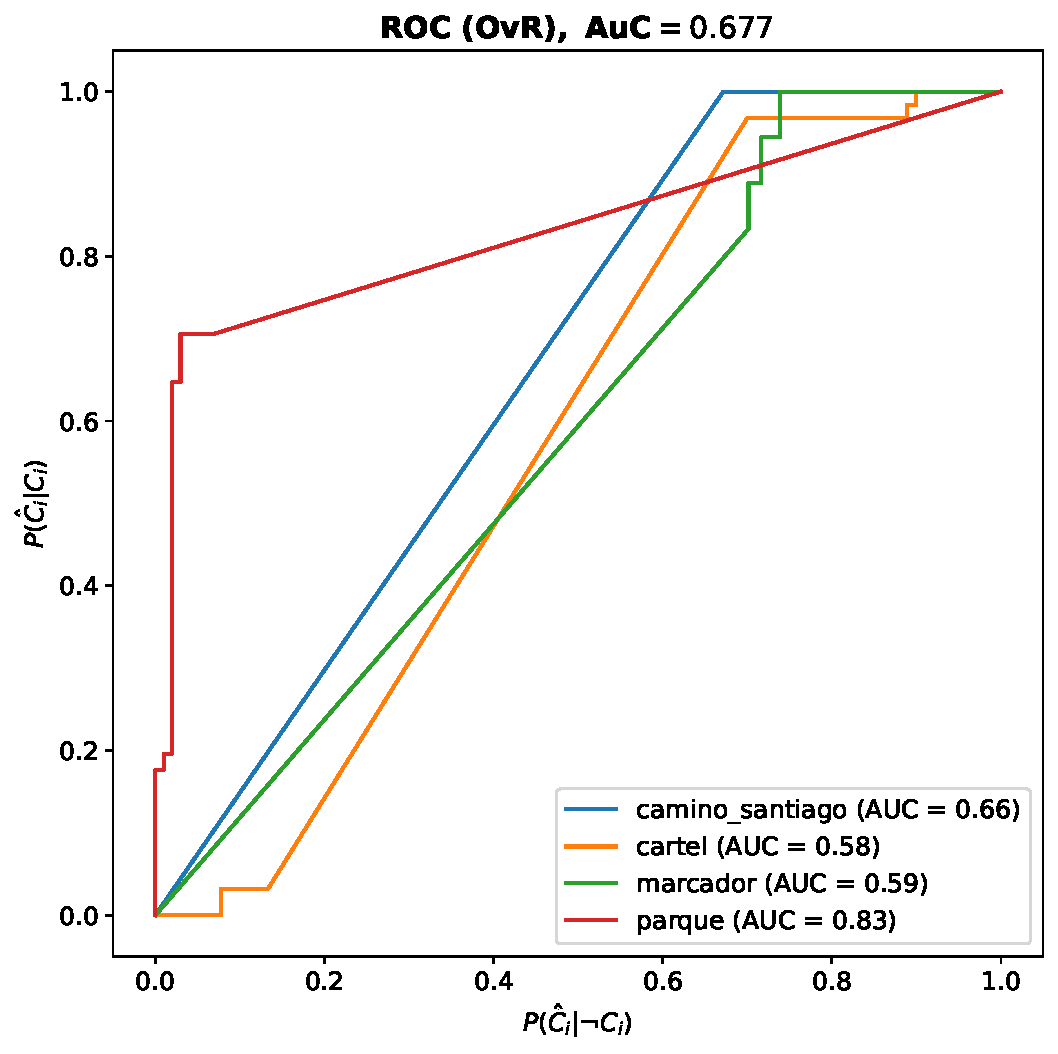
\includegraphics[scale = .5]{auc_conv}
						\caption{Normal}
						\label{fig:roc_conv}
					\end{subfigure}\hfill
					\begin{subfigure}{.4\textwidth}
						\centering
						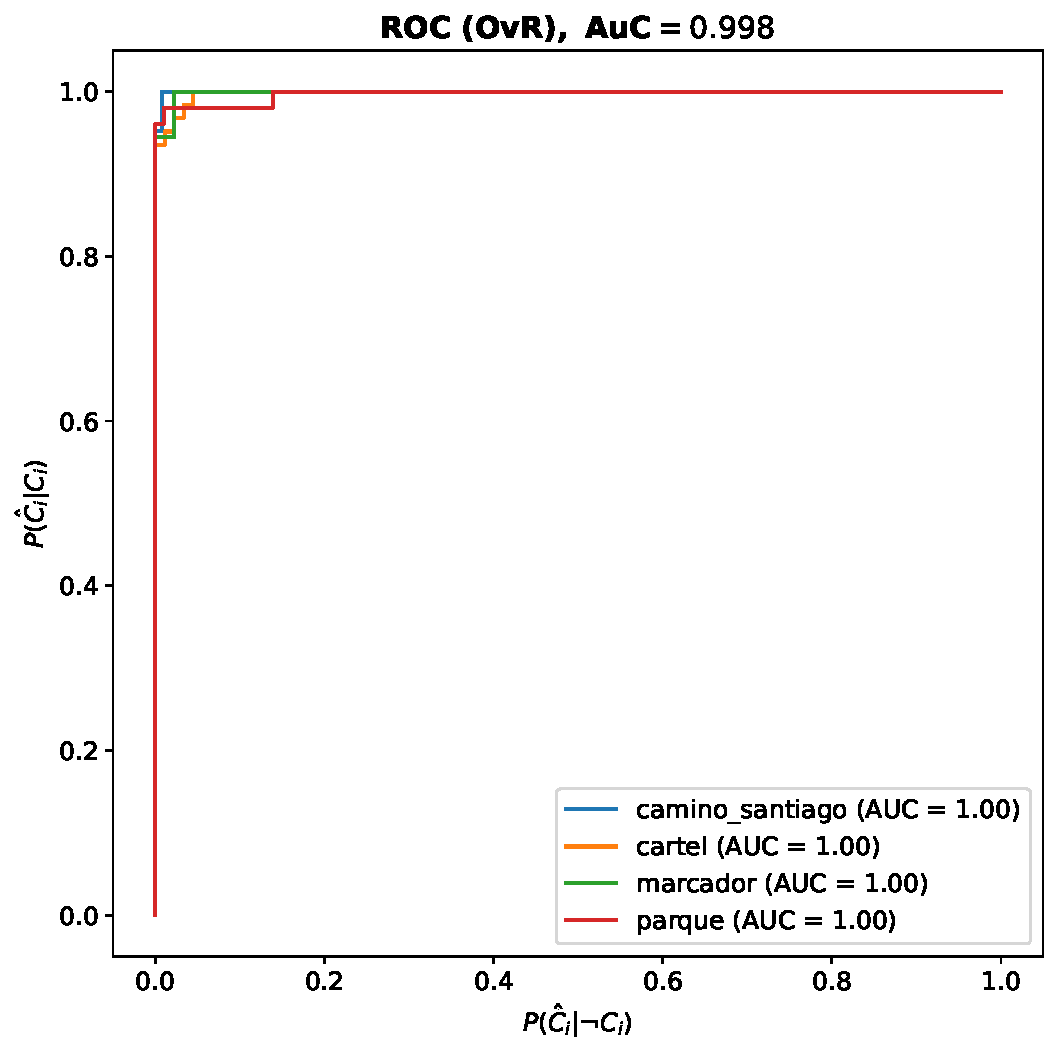
\includegraphics[scale = .5]{auc_mb}
						\caption{Aplicando transfer learning}
						\label{fig:roc_mb}
					\end{subfigure}
					\begin{subfigure}{.4\textwidth}
						\centering
						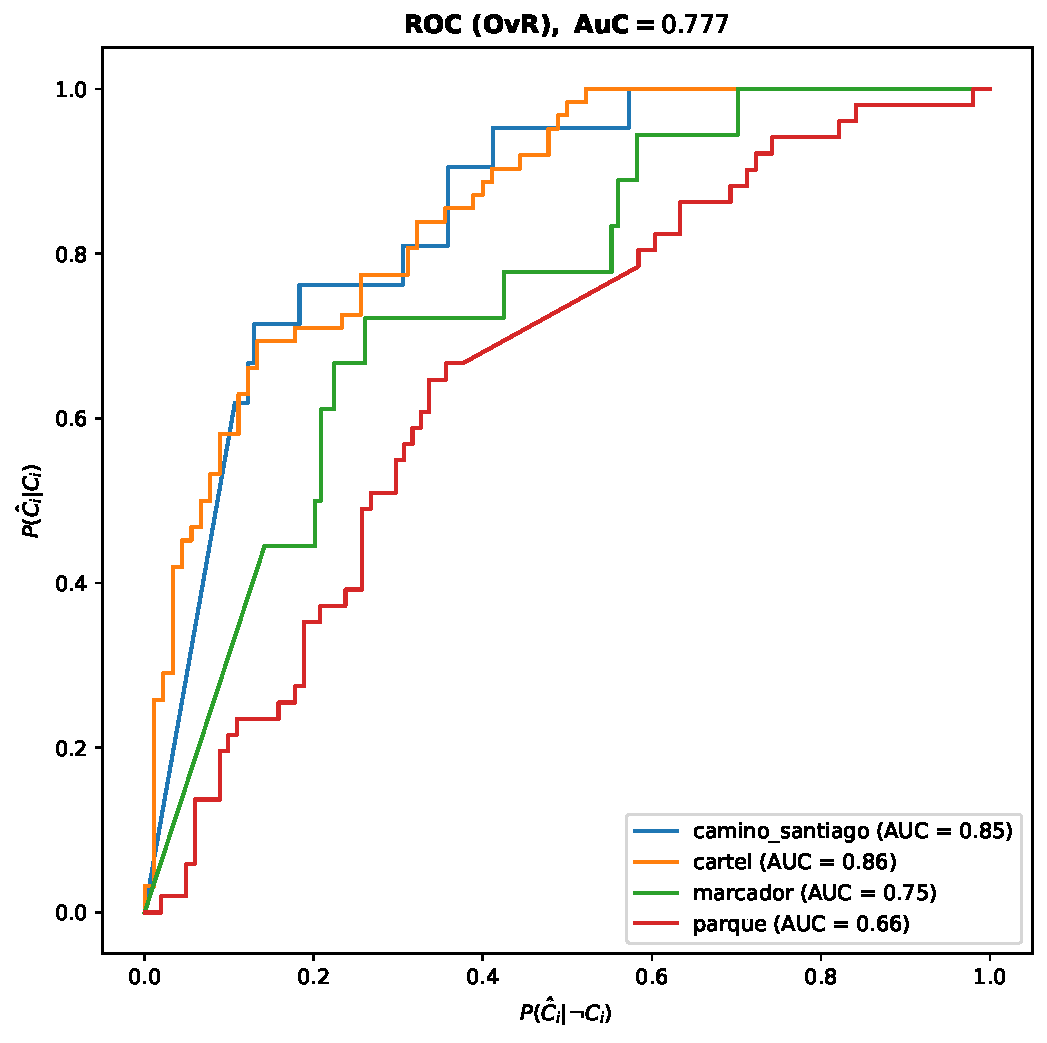
\includegraphics[scale = .5]{auc_convau}
						\caption{Aplicando aumento de datos}
						\label{fig:roc_convau}
					\end{subfigure}\hfill
					\begin{subfigure}{.4\textwidth}
						\centering
						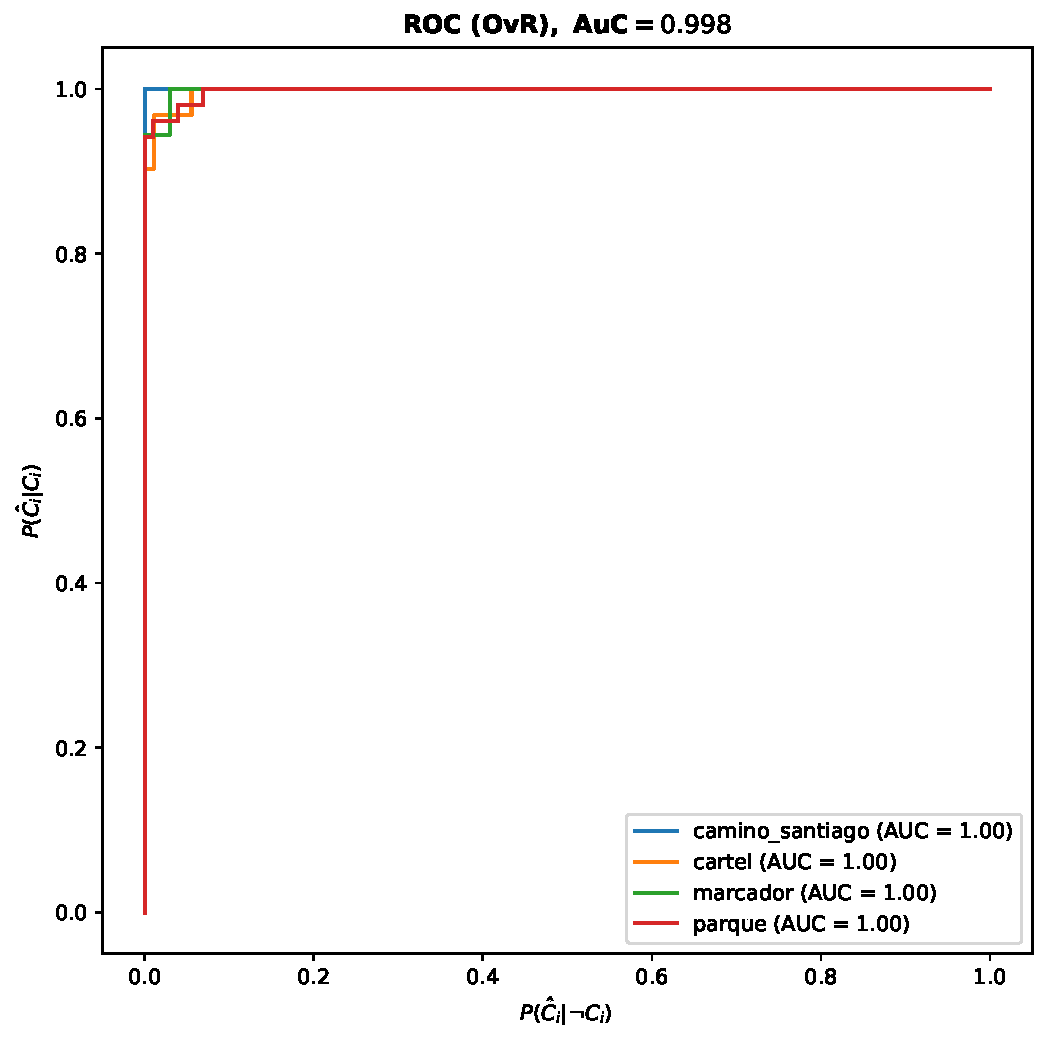
\includegraphics[scale = .5]{auc_mbau}
						\caption{Aplicando ambas}
						\label{fig:roc_mbau}
					\end{subfigure}
					\caption{Curvas ROC}
					\label{fig:roc}
				\end{figure}
			
				Como resumen de esta parte, se puede concluir que el entrenamiento de una red convolucional desde cero es un proceso complejo y que requiere de una cantidad enorme de datos, que en los casos en los que no se dispone de ellos, conduce a resultados negativos, siendo necesario aplicar la técnica de transfer learning. A pesar de haber visto su gran eficacia, se va a realizar una prueba más. \\
				
				El dataset empleado, contenía imágenes de diferentes partes de España, por lo que el modelo estaba viendo variantes de cada tipo de objeto. Lo que se va a hacer ahora es separar dicho dataset de manera que contenga únicamente en el conjunto de test imágenes de la ciudad de Guadalajara. Al ser pocas, el experimento no será muy representativo, pero permitirá probar la eficacia de la red generalizando conceptos. Para ello se ha utilizado el mismo modelo que se ha utilizado en el caso de transfer learning (entrenando de nuevo los parámetros desde cero para evitar hacer predicciones de una imagen vista durante el entrenamiento). \\
				
				\begin{figure}[!h]
					\centering
					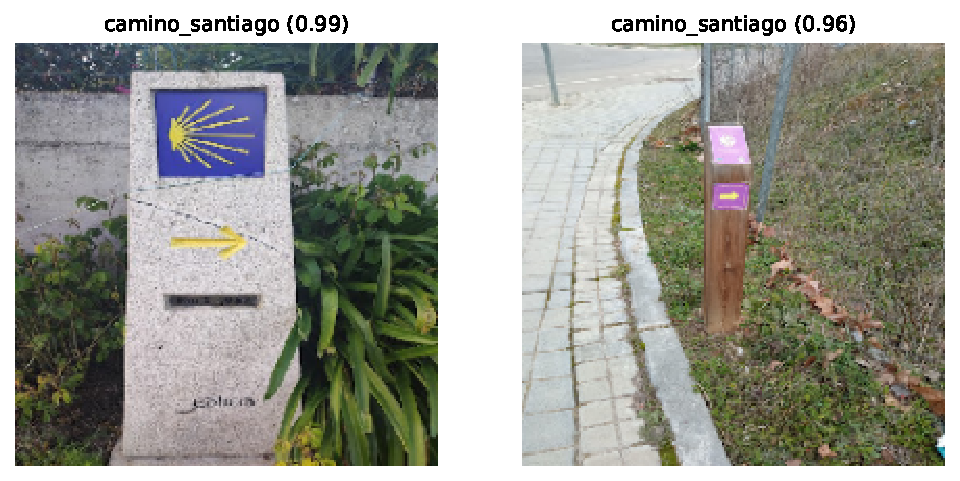
\includegraphics[scale = .8]{gu_vs_ga}
					\caption{Experimento de la capacidad de generalización de la red}
					\label{fig:comparativa_gu}
				\end{figure}
				
				Como se observa en la \Cref{fig:comparativa_gu}, tras haber entrenado el modelo sin usar imágenes de objetos de Guadalajara, y enseñarle uno como por ejemplo este hito del Camino de Santiago, la red está casi segura que de uno de ellos se trata, a pesar de que sea completamente distinto a los que ha visto durante el entrenamiento con el aspecto típico de Galicia. 
	
	\paginavacia
	\addcontentsline{toc}{chapter}{Bibliografía}
	\pagestyle{plain}
	\printbibliography
	
	% CONTRAPORTADA
	\chapter*{}
	\thispagestyle{empty}
	\cleartoleftpage
	\thispagestyle{empty}
	\BgThispage
	
	\begin{tikzpicture}[remember picture,overlay]
		\node[yshift = -5cm] at (current page.north west){
			\begin{tikzpicture}[remember picture, overlay]
				\draw[fill = headingPortadaTFG, headingPortadaTFG] (0,0) rectangle (\paperwidth,5cm);
				\node[yshift = 3cm, xshift = 0.5\paperwidth, font = \Huge, text centered, midway] {\color{textoHeadingPortadaTFG}\universidad};
				\node[yshift = 2cm, xshift = 0.5\paperwidth, font = \Huge, text centered, midway] {\color{textoHeadingPortadaTFG}\escuela};
			\end{tikzpicture}
		};
	\end{tikzpicture}
	
	\large
	\vspace{19.3cm}
	
	\begin{center}
		\centerline{
			
\includegraphics[height=2.5cm]{01_logo-vA_pant293.pdf}
		}
	\end{center}
	
\end{document}